\chapter{Spatially shifting temporal points: estimating pooled within-time series variograms for scarce hydrological data}
\label{chapter3}

Avit Kumar Bhowmik\textsuperscript{a} and Pedro Cabral\textsuperscript{b}\\[.5cm]
\small
\textsuperscript{a}Quantitative Landscape Ecology, Institute for Environmental Sciences, University of Koblenz-Landau, Fortstraße 7, 76829 Landau in der Pfalz, Germany\\
\textsuperscript{b}NOVA Information Management School, Universidade Nova de Lisboa, Campus de Campolide, 1070-312 Lisboa, Portugal\\[1cm]

\normalsize

Adapted from the article under review in Hydrology and Earth System Sciences (HESS)\footnote{HESS is ranked 2\textsuperscript{nd} in the field of water resources research. The current impact factor of the journal is 3.535 according to the Journal Citation Reports, 2015 (\href{http://wokinfo.com/products_tools/analytical/jcr/#}{http://wokinfo.com/products\textunderscore tools/analytical/jcr/#})} and published in 2015 in Hydrology and Earth System Sciences Discussions (HESSD)\footnote{Papers under review in HESS are published as discussion papers and archived in HESSD after the review by an editor}, vol. 12, pp 2243-2265.\\[.5cm]

\renewcommand{\abstractname}{Abstract}
\begin{abstract}
Estimation of pooled within-time series (PTS) variograms is a frequently used technique for geostatistical interpolation of continuous hydrological variables in spatially data-scarce regions. The only available method for estimating PTS variograms, i.e. averaging empirical variograms (AEV), estimationdoes not account for the varying numbers and locations of spatial data points in a time series. Here, we outlined an alternative method, i.e. spatially shifting temporal points (SSTP), for estimating PTS variograms by spatializing temporal data points and shifting them. The data were pooled by ensuring consistency of spatial structure and temporal stationarity within a time series, while pooling sufficient number of data points and increased data density for reliable variogram estimation. The pooled spatial data point sets from different time steps were assigned to different coordinate clusters on the same space. Then a semivariance was computed for each spatial-lag by simultaneously comparing all point pairs separable by that spatial-lag within a pooled time series, and a PTS variogram was estimated by controlling the lower and upper boundary of spatial-lags. SSTP was then applied for PTS variogram estimation of a precipitation index in Bangladesh. The precision of SSTP was compared with the available AEV and a manually modified robust, i.e. weighted AEV (WAEV) method, using weighted mean squared error (WMSE) as model-fit, and root mean squared error (RMSE) and Nash-Sutcliffe efficiency (NSE) as geostatistical interpolation performance statistics. SSTP (average WMSE: $4.54 X 10^7$, RMSE: 584.49 and NSE: 0.34) showed higher precision than the available AEV method (average WMSE: $7.52 X 10^8$, RMSE: 618.15 and NSE: 0.24), whereas showed identical precision to the WAEV method, and allowed for modelling spatial variability at $\leq$ 29 km for all time steps. SSTP was more intuitive and implemented by using the freely available R open source software environment. The method will reduce uncertainty for spatial variability modeling while preserving spatiotemporal properties of data for geostatistical interpolation of hydrological variables, particularly in spatially data-scarce developing countries.
\end{abstract}

\newpage
\thispagestyle{empty}

\vspace*{\fill}
\begin{quotation}
  \large\textit{``When you start seeing an area that was all tundra, and now all of a sudden, you see more shrubs or you see the forest encroaching, that is of great importance in terms of hydrology and ecology''}.
   ---Andrew Slater
\end{quotation}
\vspace*{\fill} 

\newpage

\section{Introduction}
\label{introduction}

Geostatistical interpolation techniques, e.g. kriging, have been extensively applied to mapping spatially continuous hydrological variables, e.g. precipitation (Carrera-Hernández and Gaskin, 2007; Durão et al., 2009; Haberlandt, 2007), stream flow (Castiglioni et al., 2011; Skøien et al., 2006; 2014), flood (Archfield et al., 2013) and runoff (Skøien et al., 2008). Modeling spatial variability, i.e. the spatial variogram, plays a central role in geostatistical interpolation (Webster and Oliver, 2007). The precision of variogram estimation strongly depends on the number of observations, i.e. spatial data points, in a region (Oliver, 2010; Truong et al., 2012). Webster and Oliver (1992; 2007) identified the threshold for satisfactorily precise isotropic and anisotropic variogram estimation as 100 and 250 data points, respectively. Moreover, variograms computed on fewer than 50 data points exhibited little precision, whereas variograms on 400 data points were computed with very high precision  (Webster and Oliver, 1992; 2007).

The number of data points in a region indicates data density, which also affects the precision of variogram estimation, and quality of kriging and other geostatisitical interpolation of hydrological variables (Parajka et al., 2015). A few data points entail a low data density and thus a high distance between data points as well as between locations of interpolation and data points. This leads to a high “smallest separation distance”, i.e. the smallest spatial-lag, between data point pairs for which empirical variograms (semivariances) are computed and thus a high uncertainty for short distant spatial variability modeling (Schuurmans et al., 2007). Moreover, the global information of the stationary hydrological variable mean becomes preponderant and leads to a loss of global variance (Bhowmik and Costa, 2014). This, in turn, leads to an overestimation and underestimation of small and large variable values, respectively.

Particularly, in developing countries, hydrological data are often scarce because of technological and economical constraints (Bhowmik, 2012; Bhowmik and Costa, 2014). Consequently, spatial variograms are often estimated with less than 50 data points and in turn the resulting variograms are mostly imprecise (Bhowmik and Cabral, 2011; Bhowmik and Costa, 2012; Castellarin, 2014; Goovaerts, 2000; Pugliese et al. 2014). Moreover, because of low data density the smallest spatial-lag is very high and hence, the uncertainty for short distant spatial variability modeling also remains high (Schuurmans et al., 2007). 

Estimation of pooled within-time series (PTS) variograms by comparing spatial variability from multiple time steps, e.g. years, that is similar to pooled within-class (or strata) variograms where spatial variability from multiple attribute classes are compared (Webster and Oliver, 2007), enables precise variogram estimation in data-scarce regions (Wagner et al., 2012). PTS variograms have been adapted to cases where the available numbers of data points and data density for individual time steps of a hydrological time series were too low to obtain satisfactory precision (Bhowmik, 2012; Rogelis and Werner, 2012; Schuurmans et al., 2007; Wagner et al., 2012). The advantages of PTS variograms over individual variograms are: (i) the number of point pairs is considerably increased, reducing the noise in empirical variograms and thus increasing the precision of variogram estimation (Rogelis and Werner, 2012), and (ii) data density can be increased and in turn the smallest spatial-lag is considerably decreased by including spatial variability from multiple time steps. For varying lengths of temporal data at different spatial points, some time steps may possess smaller spatial-lags than others. Pooling allows to include these small spatial-lags in temporally constant variogram estimation and thus to reduce uncertainties of short distant spatial variability modeling for the time steps that possess only lower data density and thus larger spatial-lags. In turn, short distant variability can be modeled for time steps with lower data density and larger spatial-lags using point pairs from time steps with higher data density and smaller spatial-lags (Schuurmans et al., 2007). Moreover, PTS variograms were shown to be more suitable than spatiotemporal variograms that are estimated for interpolation in space-time, and mean variograms that average estimated non-singular individual variogram parameters, i.e. nuggets, partial sills and ranges within time series (method d in Gräler et al. (2011)) for cases, where the spatial locations and numbers of available data points and density vary within a time series and do not meet the threshold for precise individual variogram estimation in any time step (Christakos, 2001; Kerry and Oliver, 2004). This is because temporal variability modeling is uncertain for variable spatial locations of data points and lengths of time series, and, as previously discussed, the estimated spatial variogram parameters for individual time steps are imprecise due to scarce data.

Averaging empirical variograms (AEV), which are computed by paired comparisons in individual time steps, over each spatial-lag within a pooled time series represents the only method available for PTS variogram estimation (method c in Gräler et al. (2011)). However, this method assumes the constancy of numbers and locations of spatial data points in a time series Gräler et al. (2011). The coverage of spatial data points typically increases over time in data scarce regions, particularly in developing countries and hence, time series exhibit varying numbers and locations of spatial data points (Bhowmik, 2012; Bhowmik and Costa, 2014). Therefore, the PTS variogram estimation should account for these varying numbers and locations of data points in a time series. Moreover, most studies focused on geostatistical interpolation of hydrological variables in regions with dense spatial data (Haberlandt, 2007; Skøien et al., 2006) whereas there is an increasing need for studies on spatial variability of hydrological variables in spatially data-scarce regions, particularly in developing countries (Stocker et al., 2013). Hence, only the AEV method for PTS variogram estimation is insufficient for the anticipated large number of studies on data-scarce countries.

We outline an alternative method in this paper for estimating PTS variograms by spatializing temporal data points and shifting them that automatically accounts for the varying numbers and locations of data points in a time series. We call this method “spatially shifting temporal points (SSTP)”. SSTP was developed using the freely available R (R Core Team, 2015) open source software environment. We apply SSTP to estimate PTS variograms for a hydrological series in a spatially data-scarce developing country and compare it with the AEV and a modified AEV methods.

\section{Methods}
\label{Methods}

\subsection{Spatial structure and stationarity tests}
\label{Spatial structure and stationarity tests}

Spatial structure, and spatial and temporal stationarity indicate the strength, and spatial and temporal pattern of variability of spatiotemporal variables, respectively (Kravchenko, 2003). Hence, as a PTS variogram represents a constant variability between spatial data points within a pooled time series, spatial structure requires consistency within that time series (Gräler et al., 2011). Moreover, a hydrological variable should exhibit temporal stationarity, i.e. the mean and distribution of the variable should be constant across a pooled time series (Gräler et al., 2011). The number of pooled data points should also ensure high enough precision for variogram estimation, i.e. the threshold for reliable variogram estimation (400) should be achieved (Webster and Oliver, 2007) and data density should be increased to reduce uncertainty for short-distance spatial variability modelling (Parajka et al., 2015).

We first quantified the spatial structure of  the hydrological variable in each time step by computing its spatial correlation coefficients along the longitudinal and latitudinal gradients as suggested by Kravchenko (2003). The Pettitt–Mann–Whitney test was then applied to the correlation coefficients to identify statistically significant change points within a time series and thus to identify changes in the spatial structure (Kiely et al., 1998). The (sub)time series between the change points were extracted as time series with consistent spatial structure. In a second step, we checked for the temporal stationarity of the variable within the previously extracted time series with consistent spatial structure. For the purpose, we conducted an Augmented Dickey-Fuller test for each series (Said and Dickey, 1984). The null hypothesis of the test was that the variable has a unit root in each series, where rejecting null hypothesis with statistical significance denotes temporal stationarity. In a final step, the time series with consistent spatial structure and temporal stationarity were checked to ensure that the numbers of pooled data points met the threshold for reliable variogram estimation and data density was increased. The data points of the time series that satisfied the above three criteria were pooled and used for the PTS variogram estimation. The Pettitt–Mann–Whitney test and Augmented Dickey-Fuller test were performed using the R (R Core Team, 2015) packages “cpm” (Ross, 2013) and “tseries” (Trapletti and Hornik, 2012), respectively.

Spatial stationarity, constancy of mean of a regionalized hydrological variable across a study region, is crucial for the choice of appropriate geostatistical interpolation techniques (Cressie, 1993). Hence, we checked for spatial stationarity, i.e. the presence of a trend in the mean of the regionalized hydrological variable to identify an appropraite geostatistical technique for spatial interpolation of variables. For the purpose, we identified trends (slopes) in the variable along the longitudinal and latitudinal gradients through a simple linear regression and checked for their statistical significance. Statistically significant trends in the variable indicated non-stationarity whereas trends with no statistical significance indicated stationarity.

\subsection{Computation of pooled within-time series (PTS) empirical variograms}
\label{Computation of pooled within-time series (PTS) empirical variograms}

We computed pooled within-time series (PTS) empirical variograms applying three methods: (i) Spatially shifting temporal points (SSTP) that was developed in this paper, (ii) averaging empirical variograms (AEV) that is currently the only available method and (iii) a modified AEV method, i.e. weighted AEV (WAEV) (see the schematic diagram Figure 3.1 for work-flows of the methods).

\subsubsection{Spatially shifting temporal points (SSTP)}
\label{Spatially shifting temporal points (SSTP)}

SSTP was developed in R (R Core Team, 2015) using the utilities of the “gstat” (Pebesma, 2004), “intamap” (Pebesma et al. 2011) and “spacetime” (Pebesma, 2012) packages. Data point sets from different time steps within a pooled time series were spatialized, i.e. assigned to different sets of coordinates (clusters) on the same space (Figure 3.1). Given that $s$ is a data point location vector comprised with the coordinate vector $(x,y)$, $t$ is a time vector for a pooled time series, $Z(s,t)$ is the vector for computed variable value for the data point $s$ in year $t$ and $||s_{i,t}-s{j,t}$  is the separation distance, i.e. spatial-lag of the point pair comprised with points $s_i$ and $s_j$ in year $t$, we first assigned the data points from the base year $(t_1)$ of a pooled series, e.g. 1948 of the 1948-1975 series, to its original coordinates $(x_{t_1},y_{t_1})$. Then coordinates for the data points of the latter years were calculated according to Eq. (3.1), when  $(t_1+1)+4n \leq t < (t_1+1)+4(n+1)$; $n \in N$ ($N$ = natural numbers).

\begin{figure}[t]
  \centering
  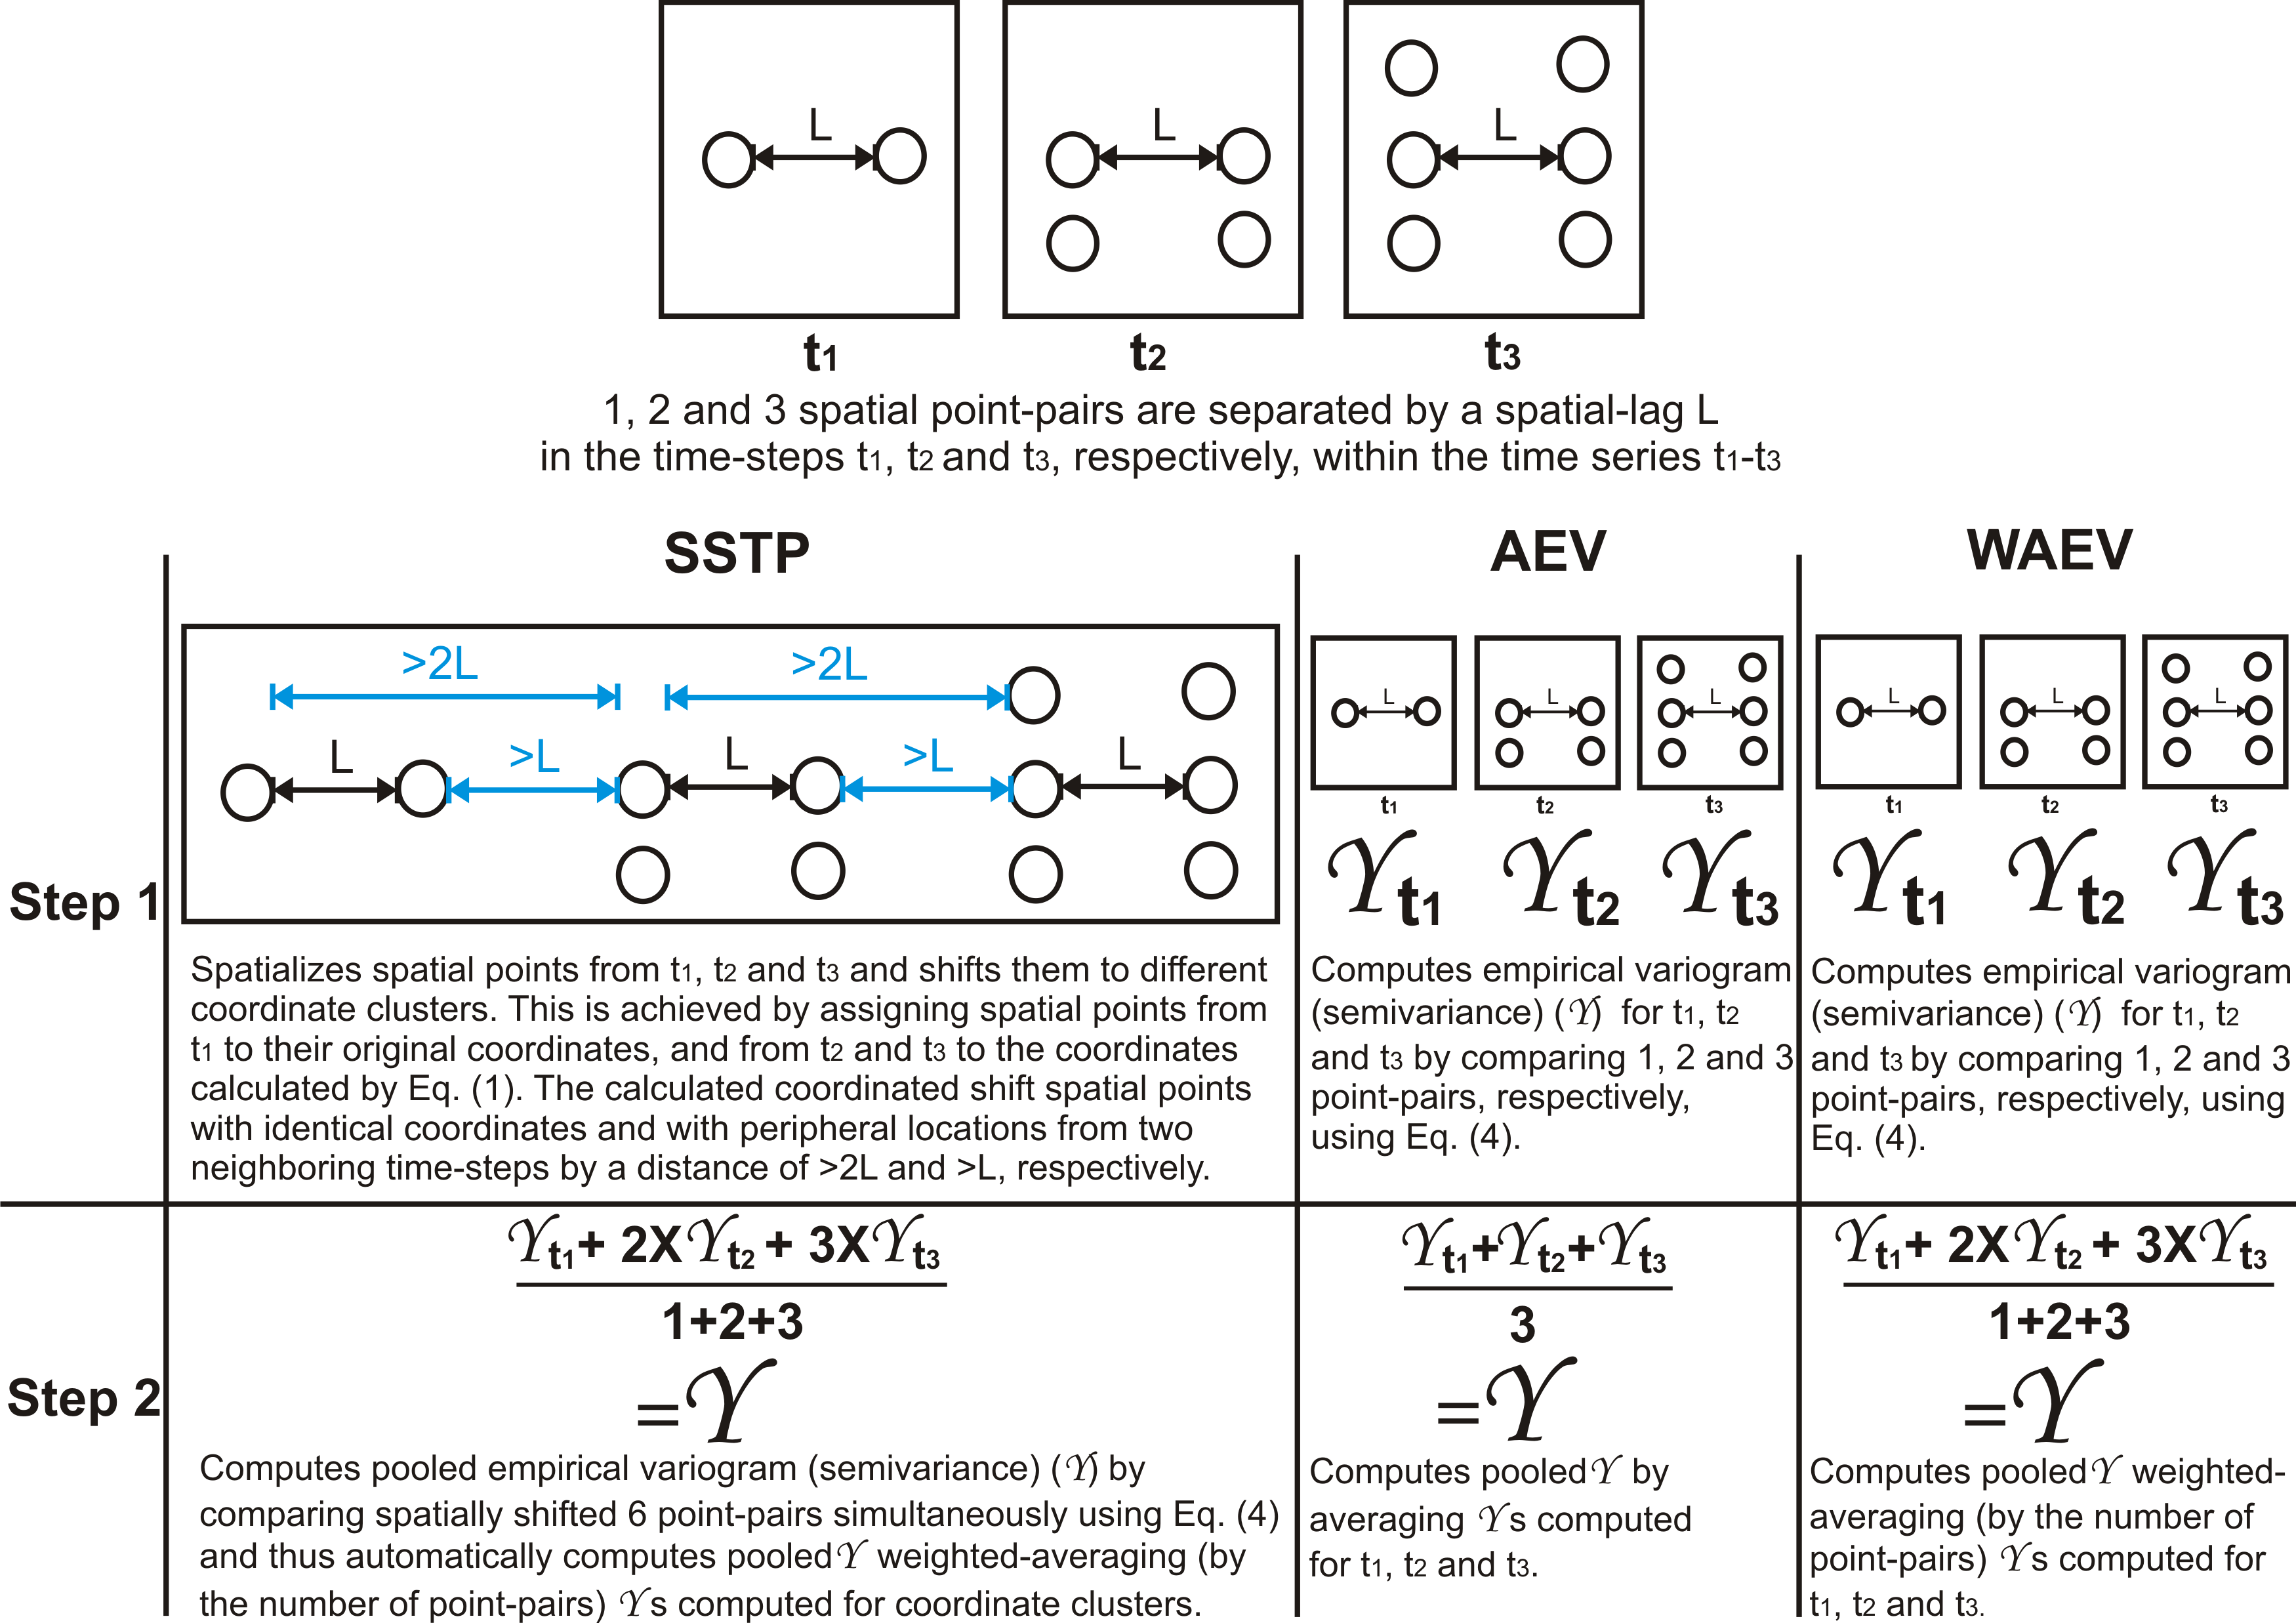
\includegraphics[width=\textwidth]{Figures/Fig_3_1.png}
  \caption{Work-flows and methodological differences between spatially shifting temporal points (SSTP), averaging empirical variograms (AEV) and weighted averaging empirical variograms (WAEV) methods for computing pooled within-time series (PTS) empirical variograms. PTS empirical variogram computation by AEV followed method c described in Gräler et al. (2011) and the method described in Pebesma and Gräler (2014).}
  \label{Fig_3_1}
\end{figure}

\begin{equation}
\begin{split}
s_{(t_1+1)+4n} = x_{(t_1+1)+4n}+(n+1)d, y_{(t_1+1)+4n} \\
s_{(t_1+1)+4n+1} = x_{(t_1+1)+4n+1}-(n+1)d, y_{(t_1+1)+4n+1} \\
s_{(t_1+1)+4n+2} = x_{(t_1+1)+4n+2}, y_{(t_1+1)+4n+2}+(n+1)d \\
s_{(t_1+1)+4n+3} = x_{(t_1+1)+4n+3}, y_{(t_1+1)+4n+3}-(n+1)d
\end{split}
\end{equation}

For example, for the years $t = {1949, 1950, 1951, 1952}$ within the pooled series of 1948-1975, $n = 0$ because   and $(1948+1)+4*0\leqt<(1948+1)+4(0+1)$ hence,

\begin{equation}
\begin{split}
s_{1949} = x_{1949}+d, y_{1949} \\
s_{1950} = x_{1950}-d, y_{1950} \\
s_{1951} = x_{1951}, y_{1951}+d \\
s_{1952} = x_{1952}, y_{1952}-d
\end{split}
\end{equation}

$d$ in Eqs. (3.1) and (3.2) is a shift distance that is bigger than two-fold the largest spatial-lag available within the pooled time series, i.e. $d>2*max||s_{i,t}-s_{j,t}||$, and shifts the data point sets of different years from each other. This shift distance was chosen because it prevents the influence of data point sets from different years on each other while estimating PTS variograms, i.e. the peripheral data points of the sets from neighboring years are separated by a distance outside of the range of the largest spatial-lag available within the pooled time series (Figure 3.1). Thus the shift distance represents a spatially rescaled temporal distancebetween data point sets from two consecutive years that preserves the spatiotemporal properties of PRCPTOT. Note that this shift distance is different from the spatially rescaled temporal distance computed for spatiotemporal variogram estimation in Gräler et al. (2011), where temporal variability was examined on a scale analogous to spatial variability. We selected the shift distance as in Eq. (3.3), but the users can choose any distance that is $>2*max||s_{i,t}-s_{j,t}||$.

\begin{equation}
d=2*max||s_{i,t}-s_{j,t}||+max||s_{i,t}-s_{j,t}||/100
\end{equation}

Spatial shifting of the temporal data points was performed using the R package “spacetime” (Pebesma, 2012). This allows for treating all temporal data points within a pooled time series as spatial points on the same space and thus for simultaneously binning and comparing point pairs from all time steps (spatial clusters) for a temporally constant spatial-lag. Moreover, point pairs from the cluster with the highest data density, where data points are separated by the smallest spatial-lag can be included in the temporally constant empirical variogram computation and thus uncertainties of short distance variability modeling for the clusters, where point pairs are only separable by larger spatial lags, are reduced.

Finally, the semivariances were computed by simulatenous comparison of all possible point pairs from the spatially shifted points using the commonly applied Methods of Moments (MoM) (Webster and Oliver, 2007). For the point pair $s_i$ and $s_j$ (both treated as spatial points on the same space), the semivariance $\gamma||s_i-s_j||$ (temporally constant) is a function of the spatial lag $||s_i-s_j||$ that is not affected by actual location of data points was computed by Eq. (3.4).

\begin{equation}
\gamma||s_i-s_j||=\frac{1}{2M||s_i-s_j||}\sum_{i,j}(Z(s_i)-Z(s_j))^2
\end{equation}

$M||s_i-s_j||$ is the number of point pairs that can be separated by the spatial lag $||s_i-s_j||$. Thus, SSTP uses a spatial variogram  computation method on the spatialized temporal points from a pooled time series and thus computes a temporally constant semivariance for each spatial-lag. In Eq. (3.4), the upper and lower boundaries of $||s_i-s_j||$ were set to the smallest and largest spatial-lags available within the pooled time series, respectively, according to Eq. (3.5).

\begin{equation}
\begin{split}
||s_i-s_j||_{smallest}=min||s_{i,t}-s_{j,t}||\\
||s_i-s_j||_{largest}=max||s_{i,t}-s{j,t}||
\end{split}
\end{equation}

These (Eq. 5) were done to reduce the uncertainty of modeling short distant spatial variability for the time steps with large spatial-lags, i.e. by modeling variability for the minimum spatial-lag within the time series (described above) and to avoid inclusion of temporal variability as pseudo spatial variability in semivariance computation, i.e. points that are temporally apart are not paired for comparison. Computation of semivariances was performed using “gstat” (Pebesma, 2004) package of R (R Core Team, 2015).

\subsubsection{Averaging empirical variograms (AEV)}
\label{Averaging empirical variograms (AEV)}

We also computed pooled semivariances using the AEV method (Figure 3.1). AEV corresponds to the method c described in Gräler et al. (2011) and the pooled variogram estimation method described in Pebesma and Gräler (2014). Semivariances for a temporally constant spatial-lag were computed for the individual time steps, where point pairs were separable by that spatial-lag. These semivariances from individual time steps were averaged to obtain the PTS semivariance.

\subsubsection{Weighted averaging empirical variograms (WAEV)}
\label{Weighted averaging empirical variograms (WAEV)}

We manually modified the AEV method for a more robust computation of pooled semivariances by taking the varying number of compared point pairs in individual time steps into account, i.e. WAEV (Figure 3.1). Semivariances for a spatial lag were computed in individual time steps as for AEV that were then averaged using a weighted approcah. The weights were provided according to the number of point pairs used for comparison in indiviual time steps.

\subsection{Test for anisotropy}
\label{Test for anisotropy}

After computation of semivariances using the above three methods, we checked for anisotropy in the spatial variability of the hydrological variable within the pooled time series. In case that anisotropy was detected, we computed the ratio between the major $(A)$ and minor $(B)$ axes of the anisotropy ellipse and the angle of the anisotropy $(\phi)$. Anisotropy parameters were computed using “intamap” package (Pebesma et al. 2011) and were converted according to the requirements of “gstat” (Pebesma, 2004) package in R (R Core team, 2015).

\subsection{Estimation and precision of PTS variograms}
\label{Estimation and precision of PTS variograms}

We estimated PTS variograms, i.e. fitted variogram models to the PTS empirical variograms for each pooled time series. Thereafter, the precision of estimated PTS variograms was evaluated by: (i) variogram model-fit to the empirical variograms and (ii) cross-validation of an appropriate kriging interpolation of the hydrological variable using the best-fit model (Webster and Oliver, 1992, 2007).

\subsubsection{Variogram model-fit}
\label{Variogram model-fit}

The available variogram models were fitted to the computed semivariances by a weighted least square approach providing $\frac{M(s_i,s_j)}{||s_i-s_j||^2}$ as weights (see Pebesma (2004) for details). However, variogram models can also be fitted by the maximum likelihood approach as described in Marchant and Lark (2007) or by providing different weights than ours if using the weighted least square approach (Pebesma, 2004). Details on the available variogram models and their formularization, and fitting in the gstat package (Pebesma, 2004) of R (R Core Team, 2015) can be found in Cressie (1983) and Pebesma (2001), respectively. The parameters of the fitted models, i.e. nugget and sill variances, and range (a) were extracted. In case that anisotropy was detected, the isotropic range parameter a was adjusted using the anisotropy parameter where geometric anisotropy was made isotropic according to Eq (3.6) through a linear transformation of coordinates with reference to the anisotropy ellipse described above (Oliver, 2010).

\begin{equation}
a=\sqrt{A^2cos^2\phi+B^2sin^2\phi}
\end{equation}

We computed the weighted mean of squared error (WMSE) as a model-fit statistic (Pebesma, 2004). The WMSEs of the previously fitted variogram models were compared and the best-fit model form with the lowest WMSE was identified for each pooled series.

\subsubsection{Kriging interpolation and performance statistics}
\label{Kriging interpolation and performance statistics}

The best-fit model form was used in a leave-one-out cross-validation of the spatial interpolation of the hydrological variable in each time step of each pooled series using an appropriate geostatistical interpolation technique, i.e. kriging. The kriging interpolation method was chosen because it gives unbiased evaluation of how well the variogram model fits the data (Oliver, 2010). The appropriate kriging technique was chosen based on the existance of spatial stationarity (described in 3.2.1) and covariates. The covariates were identified by checking spatial correlation between the hydrological variable and available other spatially dependent variables. Spatially dependent variables showing statistically significant correlation with the hydrological variable were chosen as covariates. In case that no convariate was identified and the hydrological variable showed spatial stationarity, ordinary kriging (OK) technique was used. Whereas in the presence of a trend in the regionalized variable mean, i.e. spatial non-stationarity, we used universal kriging (UK) technique. Kriging with external drift (KED) was used if covariates were available. Kriging interpolation was performed using the R (R Core Team, 2015) package “gstat” (Pebesma, 2004). For details on the kriging interpolation techniques and implementation in “gstat”, see Cressie (1983) and Pebesma (2004).

Finally, the root mean squared error (RMSE) and Nash-Sutcliffe efficiency (NSE) (Parajka et al., 2015) were computed as kriging interpolation performance statistics for each model form by comparing the observed and kriging interpolated hydrological variable values through a leave-one-out cross-validation (Pebesma, 2004). Note that we avoided the recalibration of the model form based on RMSE and NSE computed through the cross-validation because cross-validation statistics can be related to many factors other than the variogram model, such as the implementation of parameters related to the search neighborhood and used interpolation algorithm (Goovaerts, 2000).

The precision of the PTS variograms estimated by SSTP, AEV and WAEV for a pooled series were compared using correspondingWMSEs, RMSEs and NSEs.The method that estimated PTS variograms with the lowest WMSE and RMSE, and the highest NSE was chosen as the most precise variogram estimation method. To identify the effect of the consistency of spatial structure within a pooled time series on PTS variogram estimation, we also pooled the data points from a series showing inconsistent spatial structure, checked for temporal and spatial stationarity, and number and density of pooled data points and used for PTS variogram estimation. The MSEs and RMSEs, and NSEs of these PTS variograms were compared with the PTS variograms estimated for time series with consistent spatial structure.

We provide a commented R-script as a supplementary material (R\textunderscore script.R in the supplemetary material) detailing the SSTP and enabling comparison with AEV and WAEV methods for PTS variogram estimation. The sample data (Sample\textunderscore data.Rdata) for reproducibility is also provided in the supplementary material. For further modification and development of SSTP, the R-script and sample data are available from an online repository, i.e. \href{https://github.com/AvitBhowmik/SSTP}{https://github.com/AvitBhowmik/SSTP}.


\section{Study area and data}
\label{Study area and data}

The above three methods were applied to the PTS variogram estimation for “annual total precipitation in hydrological wet days (PRCPTOT)” in Bangladesh (Peterson et al., 2001) (Figure 3.2) and their precision statistics were compared. The hydrological wet days in Bangladesh refer to the monsoon season, i.e. June to September in each year, when 80 \% of the annual precipitation occurs (Bhowmik, 2012; DMICCDMP, 2012). We used the daily precipitation data from 1948-2007 series that were collected from Bangladesh Meteorological Department (DMICCDMP, 2012). Currently, 32 rain-gauges (density 2.2 rain-gauges per 10000 sq. km.) report daily precipitation in Bangladesh, classifying the country as data scarce (Webster and Oliver, 2007) (Figure 3.3). Moreover, the numbers of data points and data density exhibit an increasing coverage from 8 points in 1948 to 32 points in 2007, and from 0.5 points per 10000 sq. km in 1948 to 2.2 points per 10000 sq. km in 2007, respectively (Figure 3.3, details can be extracted from Figure B.1 and Table B.1 in appendix B). This indicates an increase in the precision of variogram estimation from 1948 to 2007. However, spatial variograms estimated for all individual years are likely imprecise as all are estimated with $<$ 50 data points and $<$ 3 points per 10000 sq. km. (Webster and Oliver, 2007) (Figure 3.3).

The precipitation data were quality controlled and validated using the “RClimdex” routine (Peterson et al., 2001). Then, PRCPTOT was computed for each of the time steps (year) and data points (rain-gauge) where precipitation data were available following the method described in Bhowmik (2012) and Peterson et al. (2001). To identify covariates, we checked for the spatial correlation between PRCPTOT and the elevation of data points.

\begin{figure}[t]
  \centering
  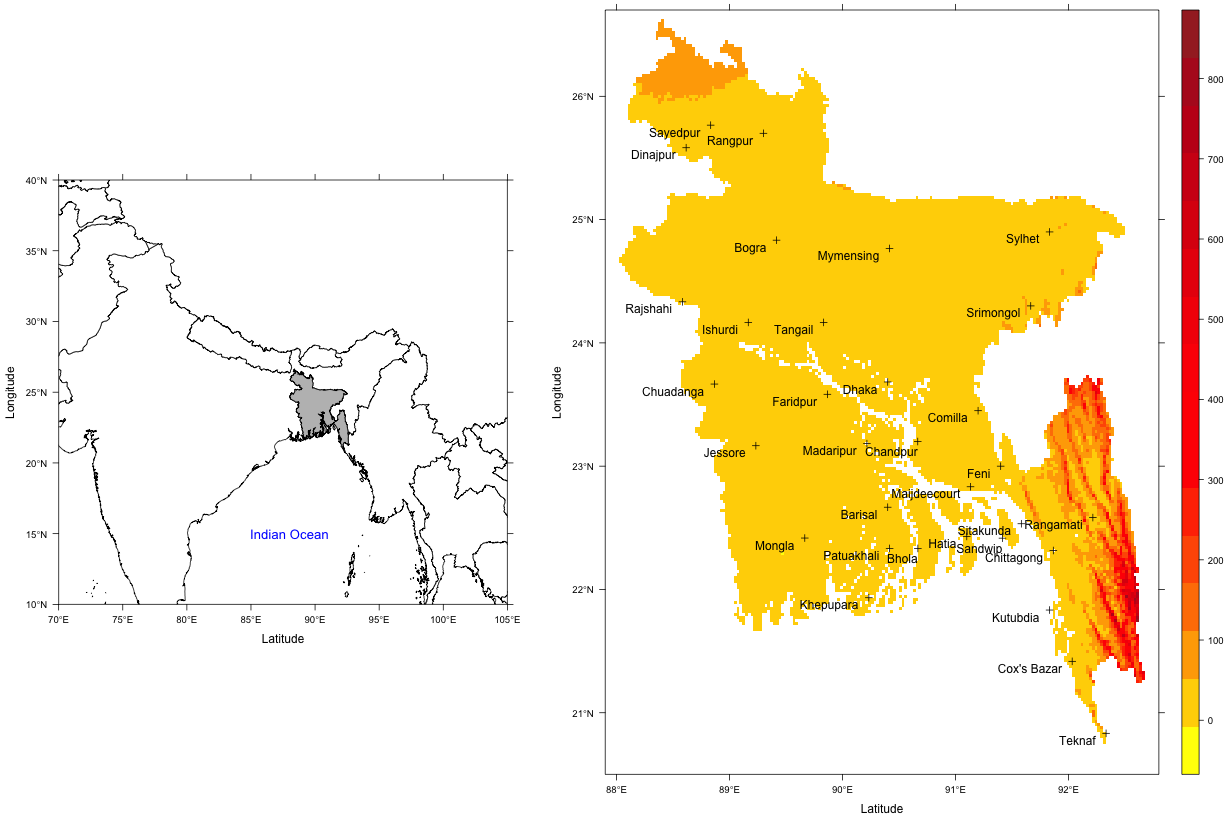
\includegraphics[width=\textwidth]{Figures/Fig_3_2.png}
  \caption{Geographic location of Bangladesh (left) in Southeast Asia within the coastal belt of Indian Ocean and the spatial distribution of currently active 32 rain-gauges (right) with altitudes (m above mean sea level) in the background. The coordinate reference system is WGS 1984.}
  \label{Fig_3_2}
\end{figure}

\begin{figure}[t]
  \centering
  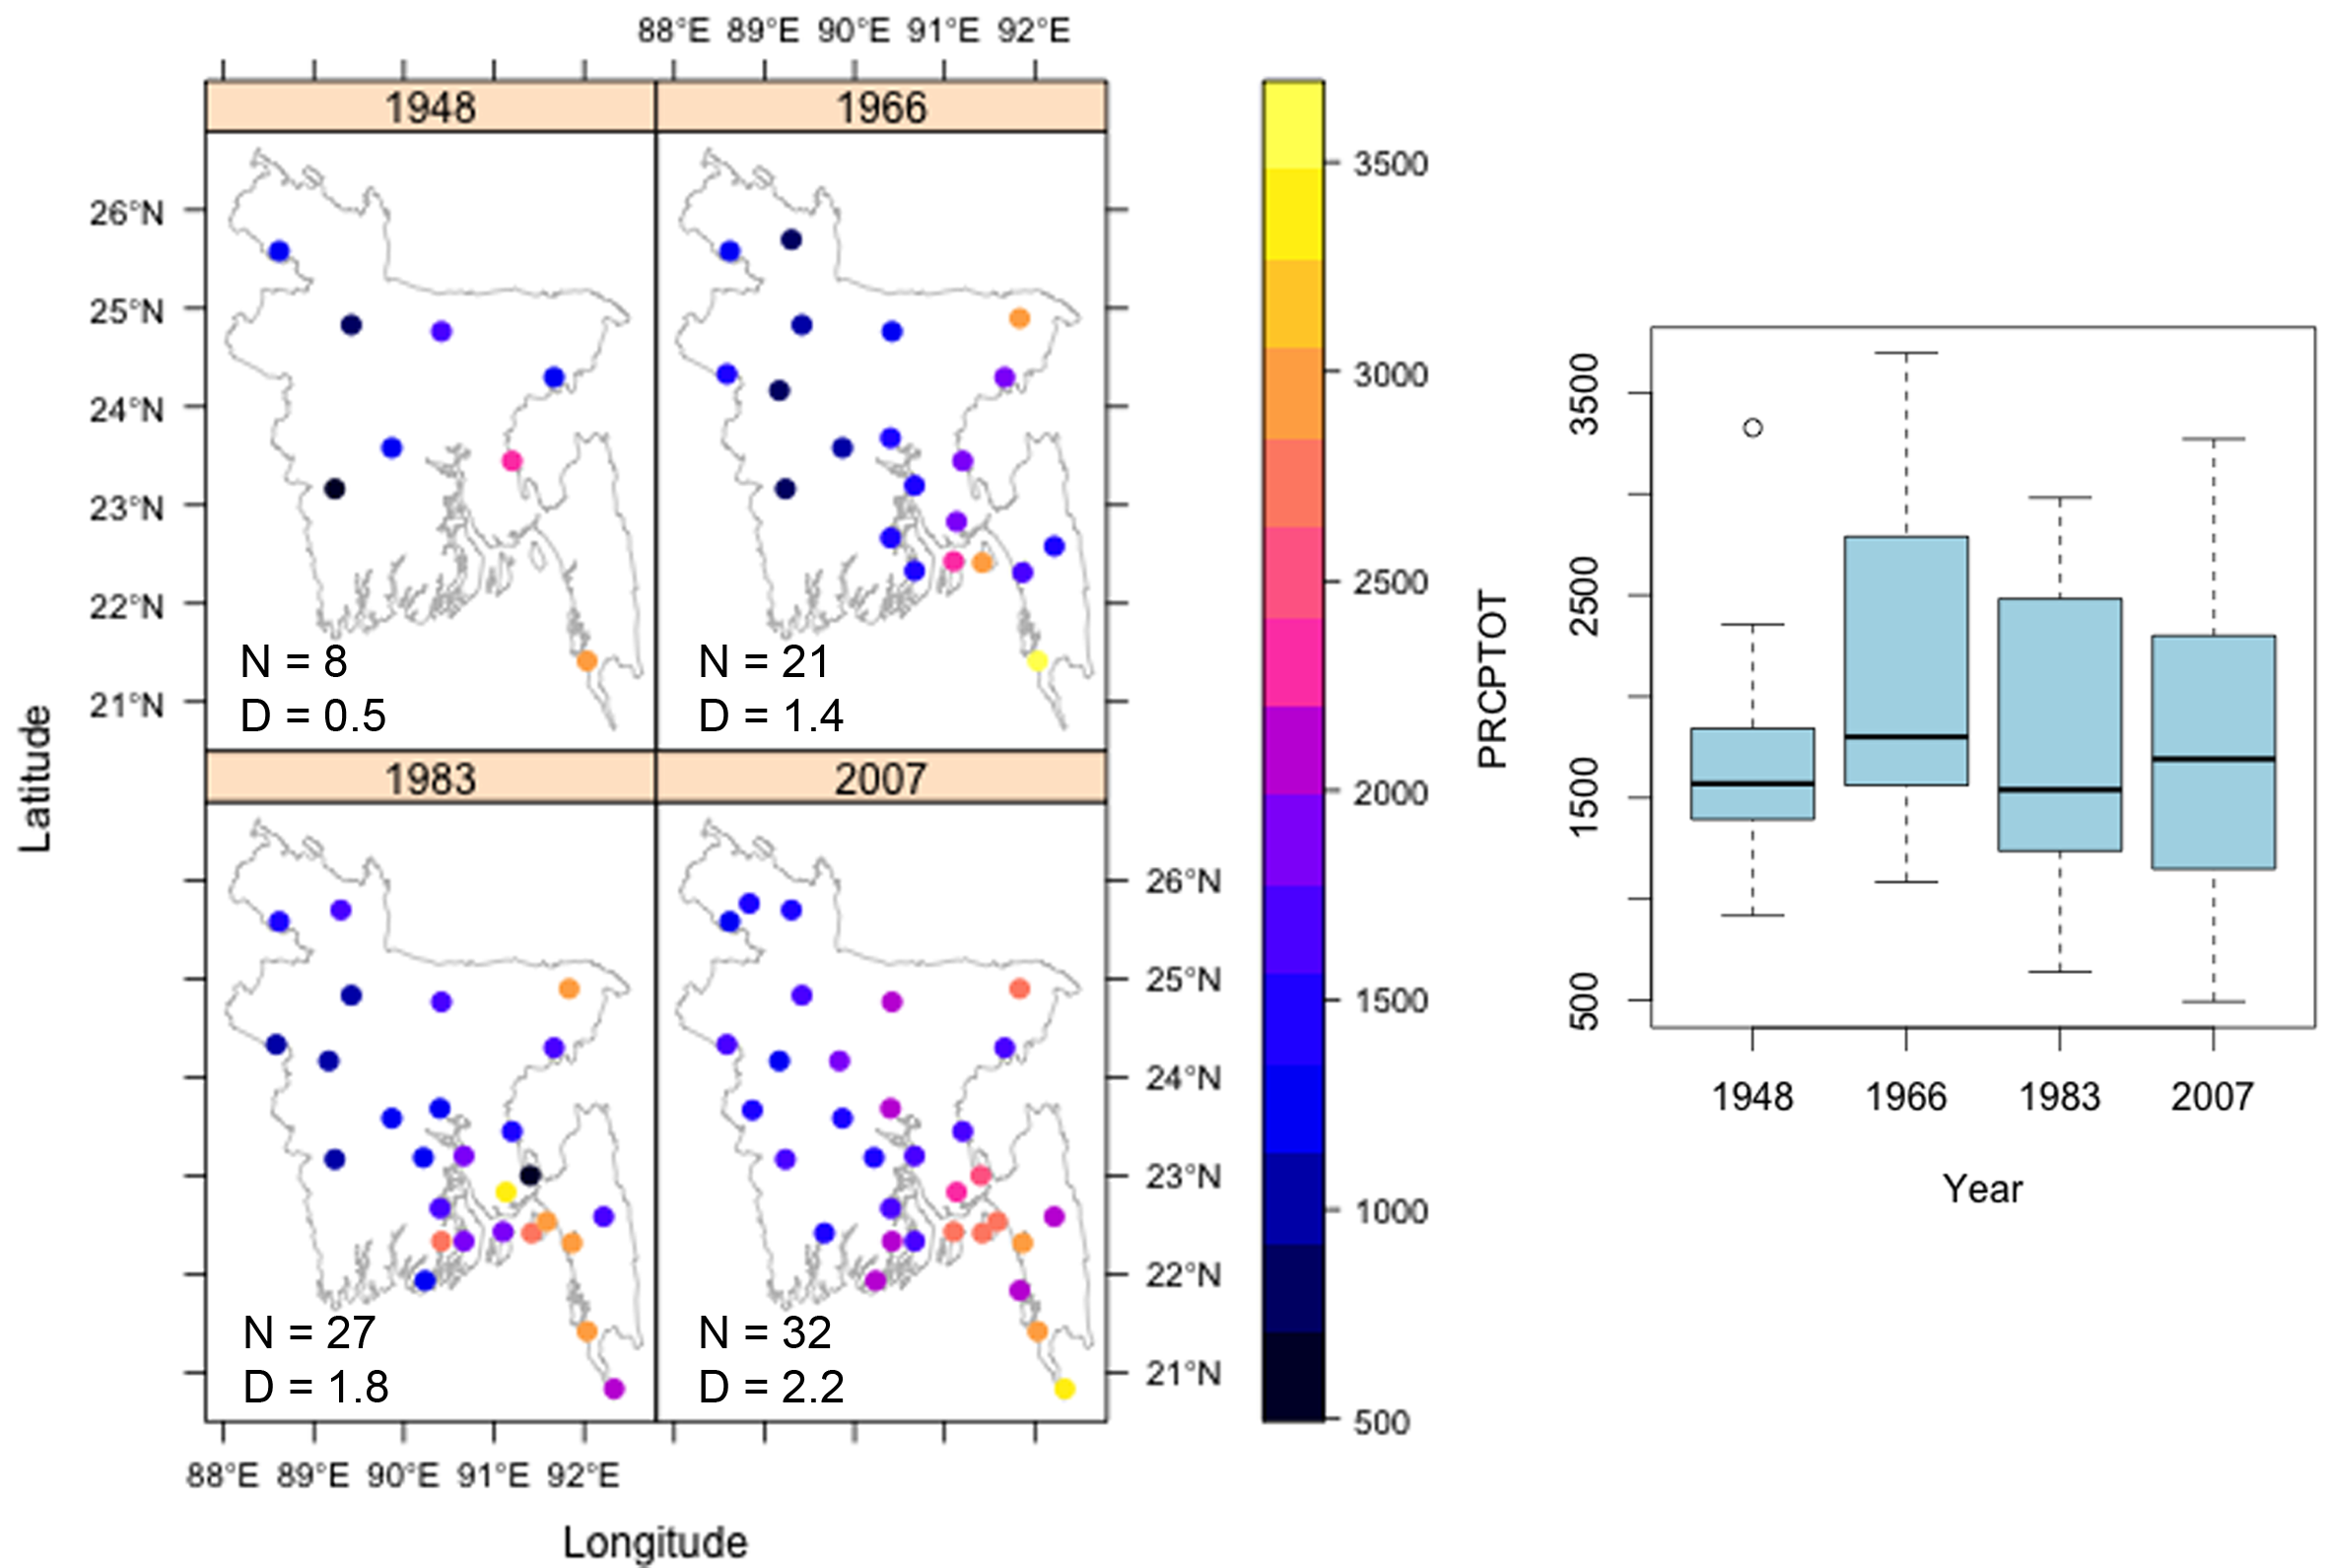
\includegraphics[width=\textwidth]{Figures/Fig_3_3.png}
  \caption{Temporally varying spatial locations, numbers (N) and density (D, in points per sq. km) of data points (left), and magnitude (in mm) and distribution of the computed annual total precipitation in hydrological wet days (PRCPTOT) (right) in Bangladesh during 1948-2007 series for four representative years, i.e. 1948, 1966, 1983 and 2007. Details on the spatial locations, N, D, magnitude and distribution of PRCPTOT in each year during 1948-2007 are available from Figure B.1 and Table B.1 in the appendix B.}
  \label{Fig_3_3}
\end{figure}

\section{Results}
\label{Results}

\subsection{Spatial structure and stationarity}
\label{Spatial structure and stationarity}

Statistically significant change points were detected in 1976 and 1993, and in 1976 for the spatial correlation coefficients of PRCOTOT along the longitudinal and latitudinal gradients, respectively, within the 1948-2007 series (Figure 3.4). These change points indicated changes in spatial structure from 1976 and 1993. Consequently, spatial structure within the entire 1948-2007 series was inconsistent whereas the (sub)time series 1948-1975, 1976-1992 and 1993-2007 showed consistent spatial structure.

\begin{figure}[t]
  \centering
  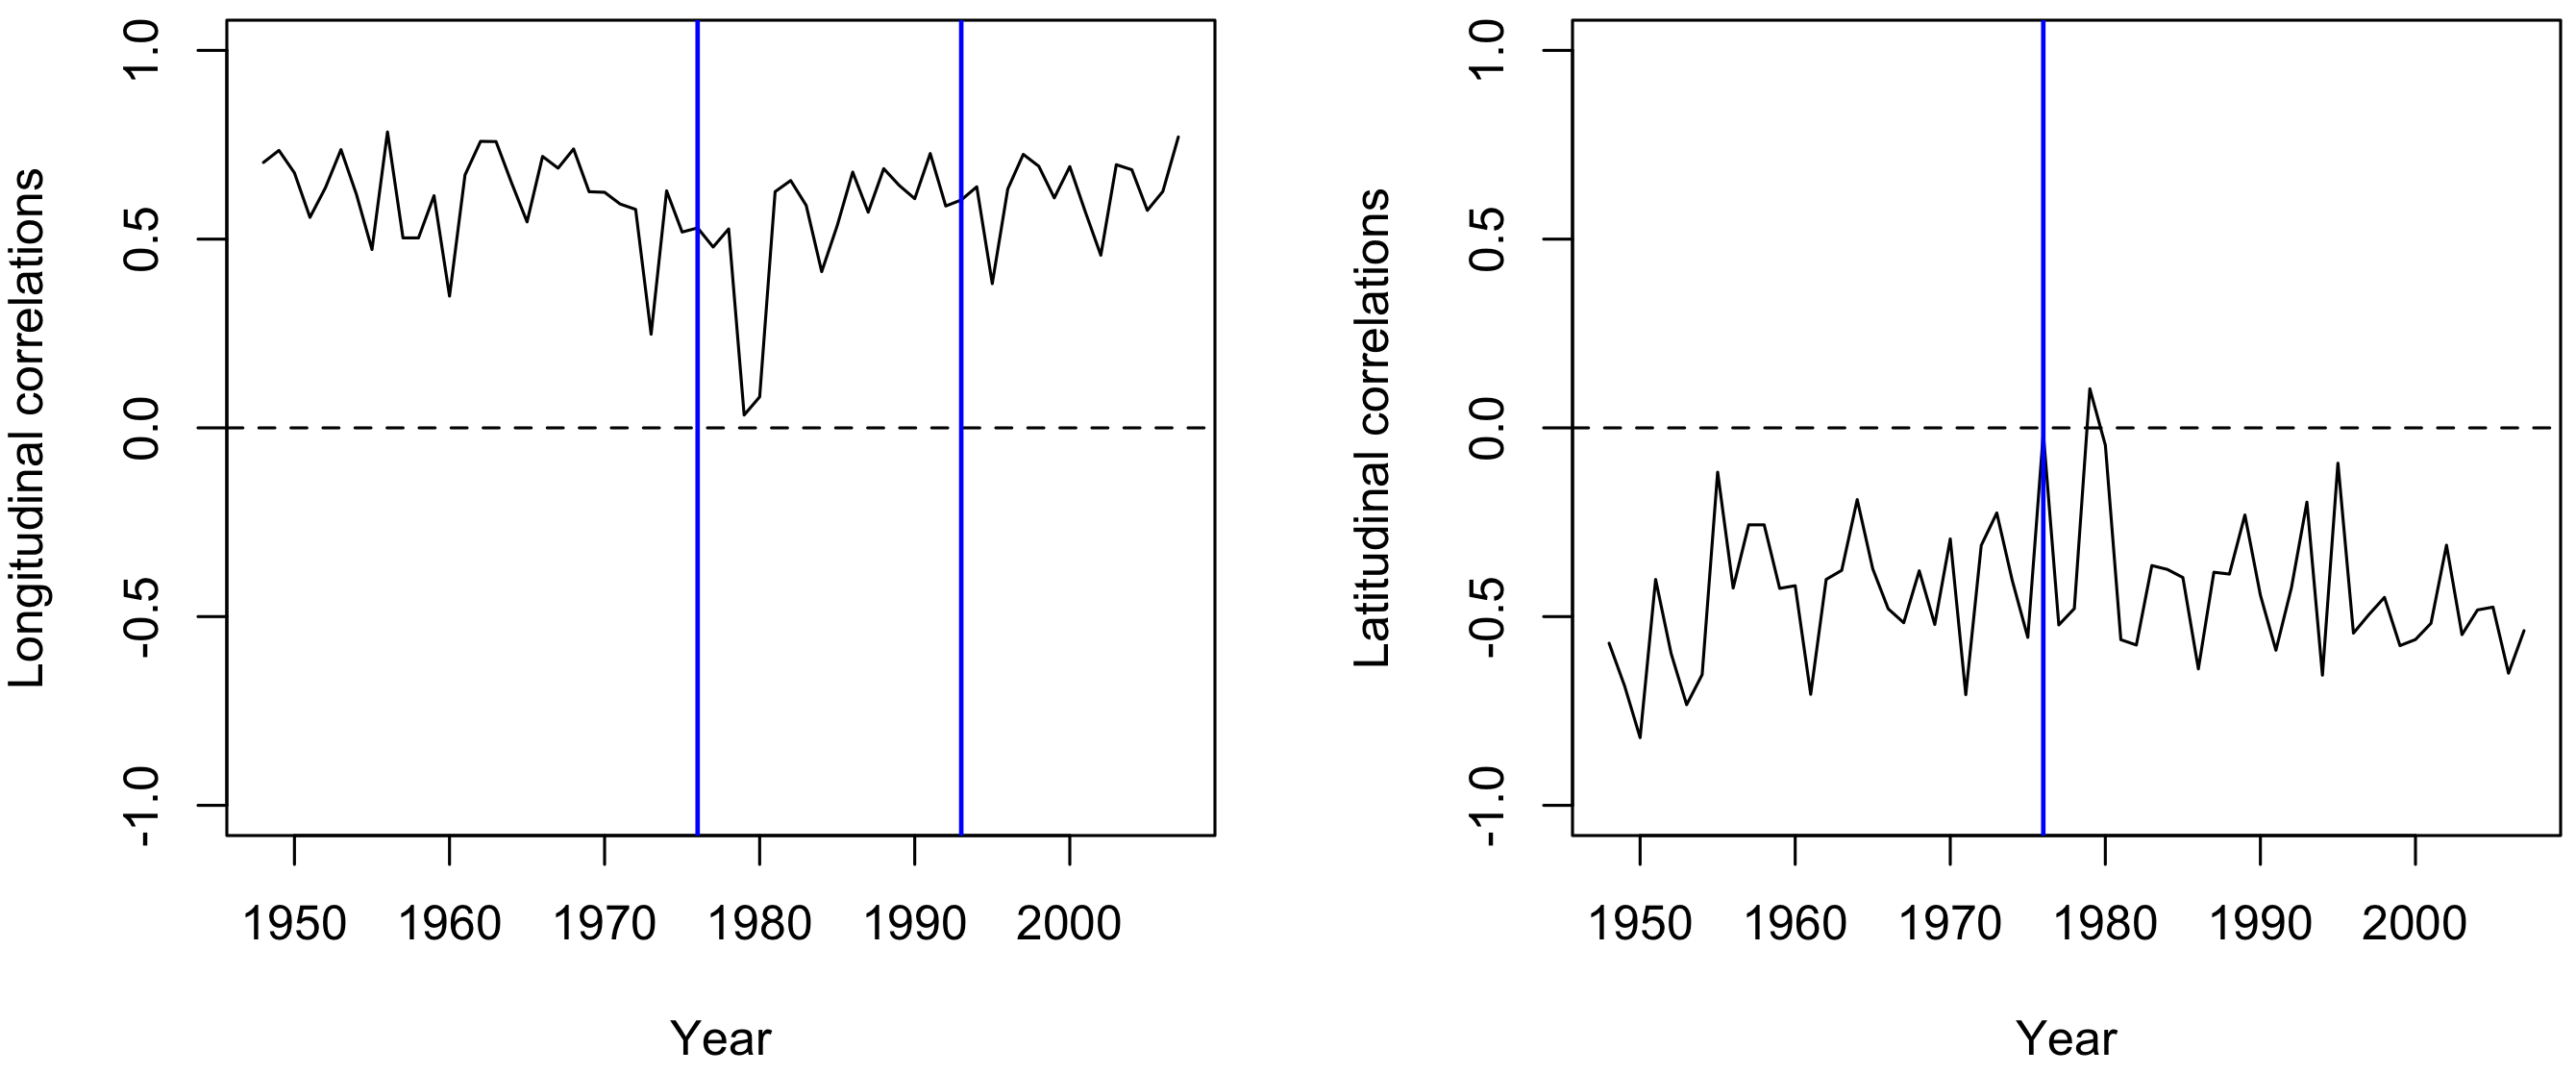
\includegraphics[width=\textwidth]{Figures/Fig_3_4.png}
  \caption{Statistically significant change points in the spatial correlations of annual total precipitation in hydrological wet days (PRCPTOT) along the longitudinal (left) and latitudinal (right) gradients within the 1948-2007 series.}
  \label{Fig_3_4}
\end{figure}

The Dickey-Fuller statistics obtained for the 1948-1972, 1976-1992, 1993-2007 and 1948-2007 series were -4.5, -3.4, -5.0 and -4.0 respectively, and they were statistically significant at p $<$ 0.01. Therefore, for each of these series null hypothesis was rejected and thus PRCPTOT showed temporal stationarity. Moreover, the number of total data points within the 1948-1975, 1976-1992, 1993-2007 and 1948-2007 series met the threshold for reliable variogram estimation (Table 3.1).

\begin{table}[h]
\label{Table 3.1}
\caption{Number of data points, smallest and largest spatial-lags, and summary statistics, i.e. minimum (Min.), mean, maximum (Max.) and coefficient of variation (CV) of annual total precipitation in hydrological wet days (PRCPTOT) within the pooled time series.}
\begin{threeparttable}
\centering
\begin{tabular}{>{\centering\arraybackslash}m{2.2cm}>{\centering\arraybackslash}m{2.0cm}>{\centering\arraybackslash}m{1.5cm}>{\centering\arraybackslash}m{1.0cm}>{\centering\arraybackslash}m{1.0cm}>{\centering\arraybackslash}m{0.7cm}>{\centering\arraybackslash}m{0.7cm}>{\centering\arraybackslash}m{0.7cm}>{\centering\arraybackslash}m{0.7cm}}

\toprule
\textbf{Pooled time series} & \textbf{Number of pooled data points} & \textbf{Data density} & \multicolumn{2}{c}{\textbf{Spatial lag}} & \multicolumn{4}{c}{\textbf{PRCPTOT}}\\
 & & & \textbf{Smallest} & \textbf{Largest} & \textbf{Min.} & \textbf{Mean} & \textbf{Max.} & \textbf{CV}\\
 & & \textbf{(point/10000 $km^2$)} & \textbf{$(km)$} & \textbf{$(km)$} & \textbf{$(mm)$} & \textbf{$(mm)$} & \textbf{$(mm)$} & \textbf{(\%)}\\

\midrule

1948-1975 & 441 & 1.5 & 29.16 & 550 & 17 & 1659 & 4036 & 42\\
1976-1992 & 465 & 2.2 & 26.61 & 550 & 84 & 1759 & 4499 & 42\\
1993-2007 & 475 & 2.2 & 27.51 & 550 & 29 & 1789 & 4516 & 41\\
1948-2007* & 1381 & 2.2 & 26.61 & 550 & 17 & 1738 & 4516 & 41\\

\bottomrule

\end{tabular}
\begin{tablenotes}
\footnotesize
* Pooled time series with inconsistent spatial structure
\end{tablenotes}
\end{threeparttable}
\end{table}

Statistically significant positive and negative spatial trends were observed in PRCPTOT along the logitudinal (363.90 mm/0, p $<$ 0.001) and latitudinal (-246.73 mm/0, p $<$ 0.001) gradients. Therefore, regionaliged PRCPTOT depicted trend in the mean and hence, exhibited spatial non-stationarity. This is also supported by Figure 3.3, where a gradual increase in PRCPTOT was observed from the Northwest to Southeast of Bangladesh. 

\subsection{Pooled within-time series (PTS) empirical variograms}
\label{Pooled within-time series (PTS) empirical variograms}

\subsubsection{Spatial shifts}
\label{Spatial shifts}

The distance $d$ used for spatial shifting by spatially shifting temporal points (SSTP) method in each of the pooled series was 1111 km ($~10^0$, decimal degree as a geographical measure of longitude or latitude with WGS 1984 datum) because the largest spatial-lag available within these series was approximately 550 km ($~5^0$) (Figure 3.5; Table 3.1). Thus the shifted peripheral data points sets from neighboring years showed a distance $>$ 550 km, i.e. $\geq$ (1111-550) km (Figure 3.5), and therefore the spatiotemporal properties of PRCPTOT were preserved, i.e. the data points from a year did not influence data points from other years and temporal autocorrelation was coherent with the spatial autocorrelation of the spatialized point clusters (Figure 3.5). Consequently, the shift distance represents a spatially rescaled temporal distance (1 year) between data point sets from two consecutive years that preserves the spatiotemporal properties of PRCPTOT.

\subsubsection{Empirical variograms}
\label{Empirical variograms}

SSTP computed a single temporally constant semivariance of PRCPTOT for each spatial-lag by simultaneously comparing point pairs from all years that are separable by that spatial-lag (Figure 3.5; 3.6). For example, for the pooled series of 1948-1975, point pairs with PRCPTOT observations that were separated by 100 km in each of the 25 clusters could be binned and compared simultaneously for a single empirical variogram computation (Figure 3.5; 3.6). Consequently, the number of point pairs for comparison could be increased to 441 as they were pooled from 25 clusters (years) (Table 3.1). Departing from SSTP, the averaging empirical variograms (AEV) and weighted AEV (WAEV) methods computed yearly semivariances for each spatial lag, i.e. computed separate semivariance for each SSTP coordinate cluster, and averaged them arithmatically and weighting by the number of comapred point pairs in each cluster, respectively. Consequently, the SSTP and WAEV computed semivariances were much less noisy than the semivariances computed by AEV, especially for large spatial-lags (Figure 3.6).

\subsubsection{Data density and short distance variabiity}
\label{Data density and short distance variabiity}

Data density for 1948-1975 series could be increased to 1.5, and for 1976-1992, 1993-2007 and 1948-2007 to 2.2 points per 10,000 sq. km for PTS variogram estimation (Table 3.1). Consequently, the smallest spatial-lags available within the three pooled series allowed for modeling spatial variability of PRCPTOT at $\leq$ 29 km (Table 3.1). This, particularly, decreased uncertainty for short distant spatial variability modelling for the time steps where the smallest spatial-lags were substantially higher, i.e. $\geq$ 60 km for 1948-1965.

\subsubsection{Anisotropy}
\label{Anisotropy}

Anisotropy was detected in the spatial variability of PRCPTOT for all pooled series in the northwest-southeast direction ($90^0>\phi>0^0$ from normal north to anticlockwise, for details see Pebesma (2004)) indicating a strong variability of PRCPTOT in that direction (Figure 3.6). This is also coherent with the direction of spatial trend in PRCPTOT (Figure 3.3) and the strong spatial variation of PRCPTOT within the pooled time series, i.e. CV $\geq$ 41 \% (Table 3.1). Moreover, 1948-1975 series depicted weak anisotropy ($A:B=0.8$), i.e. relatively weak variability whereas 1976-1992 and 1993-2007 series depicted strong anisotropy ($A:B=0.4$), i.e. relatively strong variability (Figrue 3).

\subsection{Precision of variogram estimation}
\label{Precision of variogram estimation}

\subsubsection{Variogram model-fit}
\label{Variogram model-fit}

The “Power” (Pow) model showed the best fit, i.e. the lowest weighted mean of squared error (WMSE) for all methods in all pooled series (Figure 3.6). This indicates a monotonic increase in empirical variograms with an increase in the spatial-lags without reaching a threshold and hence spatial non-stationarity, which is supported by the presence of a trend in the mean of PRCPTOT (Figure 3.3).

The PTS variograms estimated by SSTP showed better model-fit (lower WMSE, i.e. $4.54 X 10^7$ on average) than the AEV (average MSE: $7.52 X 10^8$), WAEV showed identical better model-fit than AEVto SSTP (Table 3.2). The PTS variograms estimated for the time series with inconsistent spatial structure, i.e. 1948-2007, by all methods showed higher WMSE than the variograms estimated for the time series with consistent spatial structure (Table 3.2). For the time series with consistent spatial structure, WMSEs for PTS variogram estimation decreased with the increasing number of pooled data points (Table 3.2).

\begin{table}[h]
\label{Table 3.2}
\caption{Precision statistics of the pooled within-time series (PTS) variograms estimated by spatially shifting temporal points (SSTP), averaging empirical variograms (AEV) and weighted averaging empirical variograms (WAEV) methods. The weighted mean of squared errors (WMSE) as the variogram model-fit statistic, and root means squared error (RMSE) and Nash-Sutcliffe efficiency (NSE) as the universal kriging interpolation performance statistics are presented.}
\begin{threeparttable}
\centering
\begin{tabular}{>{\centering\arraybackslash}m{1.7cm}>{\centering\arraybackslash}m{1.2cm}>{\centering\arraybackslash}m{1.2cm}>{\centering\arraybackslash}m{1.2cm}>{\centering\arraybackslash}m{0.8cm}>{\centering\arraybackslash}m{0.8cm}>{\centering\arraybackslash}m{0.8cm}>{\centering\arraybackslash}m{0.7cm}>{\centering\arraybackslash}m{0.6cm}>{\centering\arraybackslash}m{0.7cm}}

\toprule
\textbf{Pooled time series} & \multicolumn{3}{c}{\textbf{WMSE}} & \multicolumn{3}{c}{\textbf{RMSE}} & \multicolumn{3}{c}{\textbf{NSE}}\\
 & \textbf{SSTP} & \textbf{AEV} & \textbf{WAEV} & \textbf{SSTP} & \textbf{AEV} & \textbf{WAEV} & \textbf{SSTP} & \textbf{AEV} & \textbf{WAEV}\\

\midrule

1948-1975 & $2.55 X 10^7$ & $6.6.3 X 10^8$ & $3.21 X 10^7$ & $622.63$ & $655.41$ & $630.58$ & $0.28$ & $0.19$ & $0.25$\\
1976-1992 & $2.47 X 10^7$ & $4.49 X 10^8$ & $3.09 X 10^7$ & $597.98$ & $653.96$ & $624.54$ & $0.30$ & $0.21$ & $0.27$\\
1993-2007 & $2.43 X 10^7$ & $3.3.4 X 10 ^8$ & $2.96 X 10^7$ & $461.50$ & $493.95$ & $485.05$ & $0.53$ & $0.47$ & $0.49$\\
1948-2007* & $1.07 X 10^8$ & $1.56 X 10^9$ & $1.15 X 10^8$ & $655.85$ & $669.29$ & $665.12$ & $0.23$ & $0.10$ & $0.18$\\

\bottomrule

\end{tabular}
\begin{tablenotes}
\footnotesize
* Pooled time series with inconsistent spatial structure
\end{tablenotes}
\end{threeparttable}
\end{table}

\subsubsection{Kriging interpolation performance}
\label{Kriging interpolation performance}

The elevation of all data points was below 50 m (Figure 3.2) and did not significantly (p = 0.8) correlate with PRCPTOT in Bangladesh. Hence, because of the unavailability of spatial convariates and presence of spatial non-stationarity, universal kriging (UK) method proved to be the most appropriate for interpolating PRCPTOT in Bangladesh.

UK interpolation of PRCPTOT fitting the PTS variogram models estimated by SSTP entailed better performance in cross-validation than AEV, showing lower root mean squared error (RMSE) and higher Nash-Sutcliffe efficiency (NSE) (Parajka et al., 2015), and identical performance to WAEV (Table 3.2). Average RMSEs and NSEs obtained for UK interpolation by fitting the PTS variograms estimated by SSTP and WAEV, and AEV  were 584.49 and 0.34, and 618.15 and 0.24, respectively. Lower RMSEs and higher NSEs were also observed for UK interpolation of PRCPTOT fitting PTS variograms estimated by all methods for the time series with consistent spatial structure than with inconsistent spatial structure (Table 3.2). Decreasing RMSEs and increasing NSEs were also observed with the increasing number of pooled data points for the time series with consistent spatial structure.

Overall, SSTP estimated PTS variograms showed better fit to the empirical variograms and data and thus showed higher precision than AEV, while showed identical precision to WAEV (Table 3.2). Moreover, higher precision in variogram estimation was obtained for the time series with consistent spatial structure than the inconsistent spatial structure, while precision increased with the increasing number of pooled data points for consistent spatial structure (Table 3.2).

\begin{figure}[h!]
  \centering
  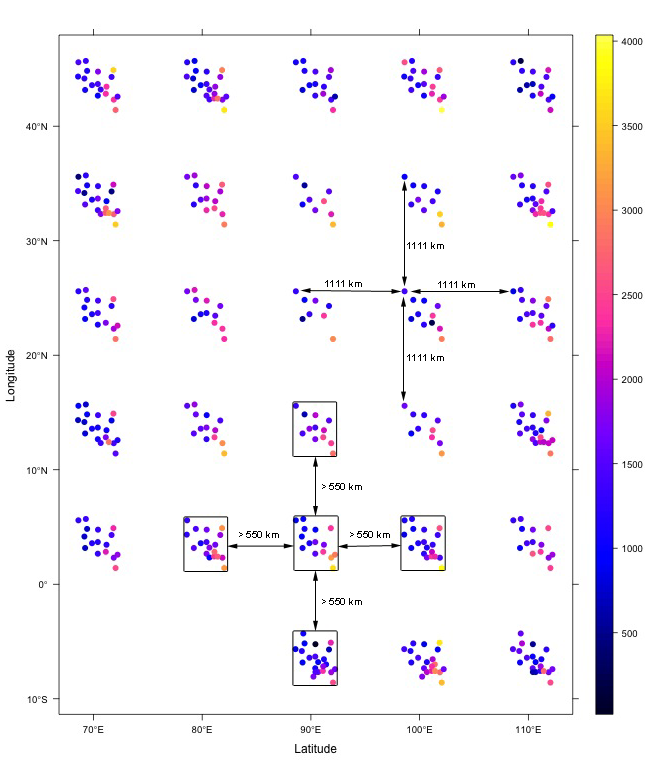
\includegraphics[width=\textwidth]{Figures/Fig_3_5.png}
  \caption{Spatially shifted (according to Eq. (1)) temporal data points for the pooled 1948-1975 series. Shift distance ($d$ = 1111 km) is calculated based on the largest-spatial-lag (550 km) available within the series (Eq. 3). The data point sets from neighboring years are shifted by 1111 km ($~10^0$), which ensures that the peripheral points of the sets are shifted by $>$ 550 km ($~5^0$). The rectangles and legend indicate peripheries (convex hull) of data points in a year and PRCPTOT in mm, respectively.}
  \label{Fig_3_5}
\end{figure}

\subsection{Discussion and future research challenges}
\label{Discussion and future research challenges}

In this paper, we developed and implemented spatially shifting temporal points (SSTP), an alternative method for estimating pooled within-time series (PTS) variograms in spatially data-scare regions. Contrasting with the available method of averaging empirical variograms (AEV)), which are computed for individual time steps, SSTP computed empirical variograms by simultaneously comparing all point pairs separable by a spatial-lag within a pooled time series (Figure 3.1; 3.6). Consequently, when compared to the PTS variograms estimated by AEV, SSTP variograms showed higher precision (Figure 3.6; Table 3.2). The numbers of available data points did not meet the threshold for satisfactorily precise variogram estimation in any of the individual time steps (year) within 1948-2007 series and data density were very low (Figure 3.3; B.1 and Table B.1). Hence, the available numbers of point pairs and smallest spatial-lags for comparisons were not sufficient for reliable semivariance computation (Webster and Oliver, 2007) (Figure 3.3). As a result, computed semivariances for the individual years were likely erratic that induced noisy and erratic semivariances when averaged by the AEV method (Figure 3.6). Thus model fitting to AEV semivariances showed a lower goodness-of-fit and universal kriging (UK) interpolation of PRCPTOT using the AEV and WAEV variogram models showed worse performance than the SSTP variograms (Figure 3.6; Table 3.2). By contrast, SSTP computed semivariances were reliable because of subtantially higher number of simultaneous comparisons and higher data density than by AEV (Table 3.1; 3.2) and thus entailed higher precision in PTS variogram estimation. These results are in line with Webster and Oliver (1992, 2007).

Semivariances computed for small spatial-lags by SSTP and AEV methods were similar whereas semivariances for large spatial-lags were largely different (Figure 3.6). Moreover, semivariances computed by AEV and WAEV showed much more noise at large spatial-lags than small spatial-lags. The number of erratic semivariances averaged by AEV for large spatial-lags were higher than for small spatial lags because point-pairs from more years were separable by large spatial-lags than by small spatial-lags due to data availability (Figure 3.3). For example, point pairs from only two years (1973 and 1975) were separable by the smallest spatial-lag for 1948-1975 series whereas point pairs from 20 years were separable by the largest spatial-lag (Table 3.1, B.1). In addition, the numbers and spatial locations of available data points are highly variable within the pooled series and spatial variability of PRCPTOT was high (Figure 3.3; Table 3.1). Hence, we argue that the averaged semivariances computed by AEV were representative of the small number of semivariances at small spatial-lags but unrepresentative of the large number of semivariances at large spatial-lags because of the variable number and spatial location of data points and high spatial variability of PRCPTOT. As a result, semivariances for large spatial-lags computed by SSTP and AEV could be similar if the numbers and spatial locations of data points were the same for all time steps and spatial variability of PRCPTOT was low (Gräler et al., 2011). However, for variable number and spatial locations of data points, the noise in the semivariances computed by AEV at large spatial-lags could be reduced by the manual modification to the robust WAEV method, i.e. by weighing the average of semivariances per spatial lag with the corresponding number of data points available per time step, and thus a better model-fit and UK interpolation performance could be achieved (Figure 3.6). Thus, SSTP automatically account for the varying numbers and locations of data points in a time series by weighting average semivariances and consequently entail identical variograms and precision to WAEV (Figure 3.1).

The PTS variograms estimated for the 1948-2007 series (inconsistent spatial structure) showed lower precision than the variograms estimated for the series with consistent spatial structure, although PRCPCTOT was stationary within 1948-2007 series, the number of data points (higher than for the series with consistent spatial structure) met the threshold for reliable variogram estimation and the highest data-density could be achieved (Webster and Oliver, 1992; 2007) (Table 3.1; 3.2). Moreover, higher precision was obtained for PTS variogram estimation with higher number of pooled data points among the series with consistent spatial structure and vice-versa (Table 3.1; 3.2). However, this may also be related to the inherent spatial structure within the time series, i.e. spatial variability of PRCPTOT may be estimated with higher precision for the data points with the spatial structure observed for 1993-2007 than for 1948-1975. Furthermore, the Hole model showed the best fit for the series with inconsistent spatial structure that did not represent the variability for individual time steps, i.e.Power variability was representative as depicted by the models for consistent spatial structure. These results suggest that the consistency of spatial structure, i.e. the strength of spatial variabilty within pooled time series is crucial for PTS variogram estimation (Kravchenko, 2003) and increasing the number of pooled data points and data density may increase the precision of PTS variogarm estimation when the spatial structure is consistent. Many studies pooled data points only by assuming the consistency of spatial structure within time series (Bhowmik, 2012; Gräler et al., 2011; Rogelis and Werner, 2012; Wagner et al., 2012). We recommend that time series should be checked for consistency of spatial structure before pooling.

The threshold for reliable variogram estimation, i.e. 400 data points (Webster and Oliver, 2007), could be achieved for each pooled series (Table 3.1). However, if data scarcity is more acute in a region and the required number of data points for reliable variogram estimation is unavailable, users

\clearpage

\begin{figure}[h!]
  \centering
  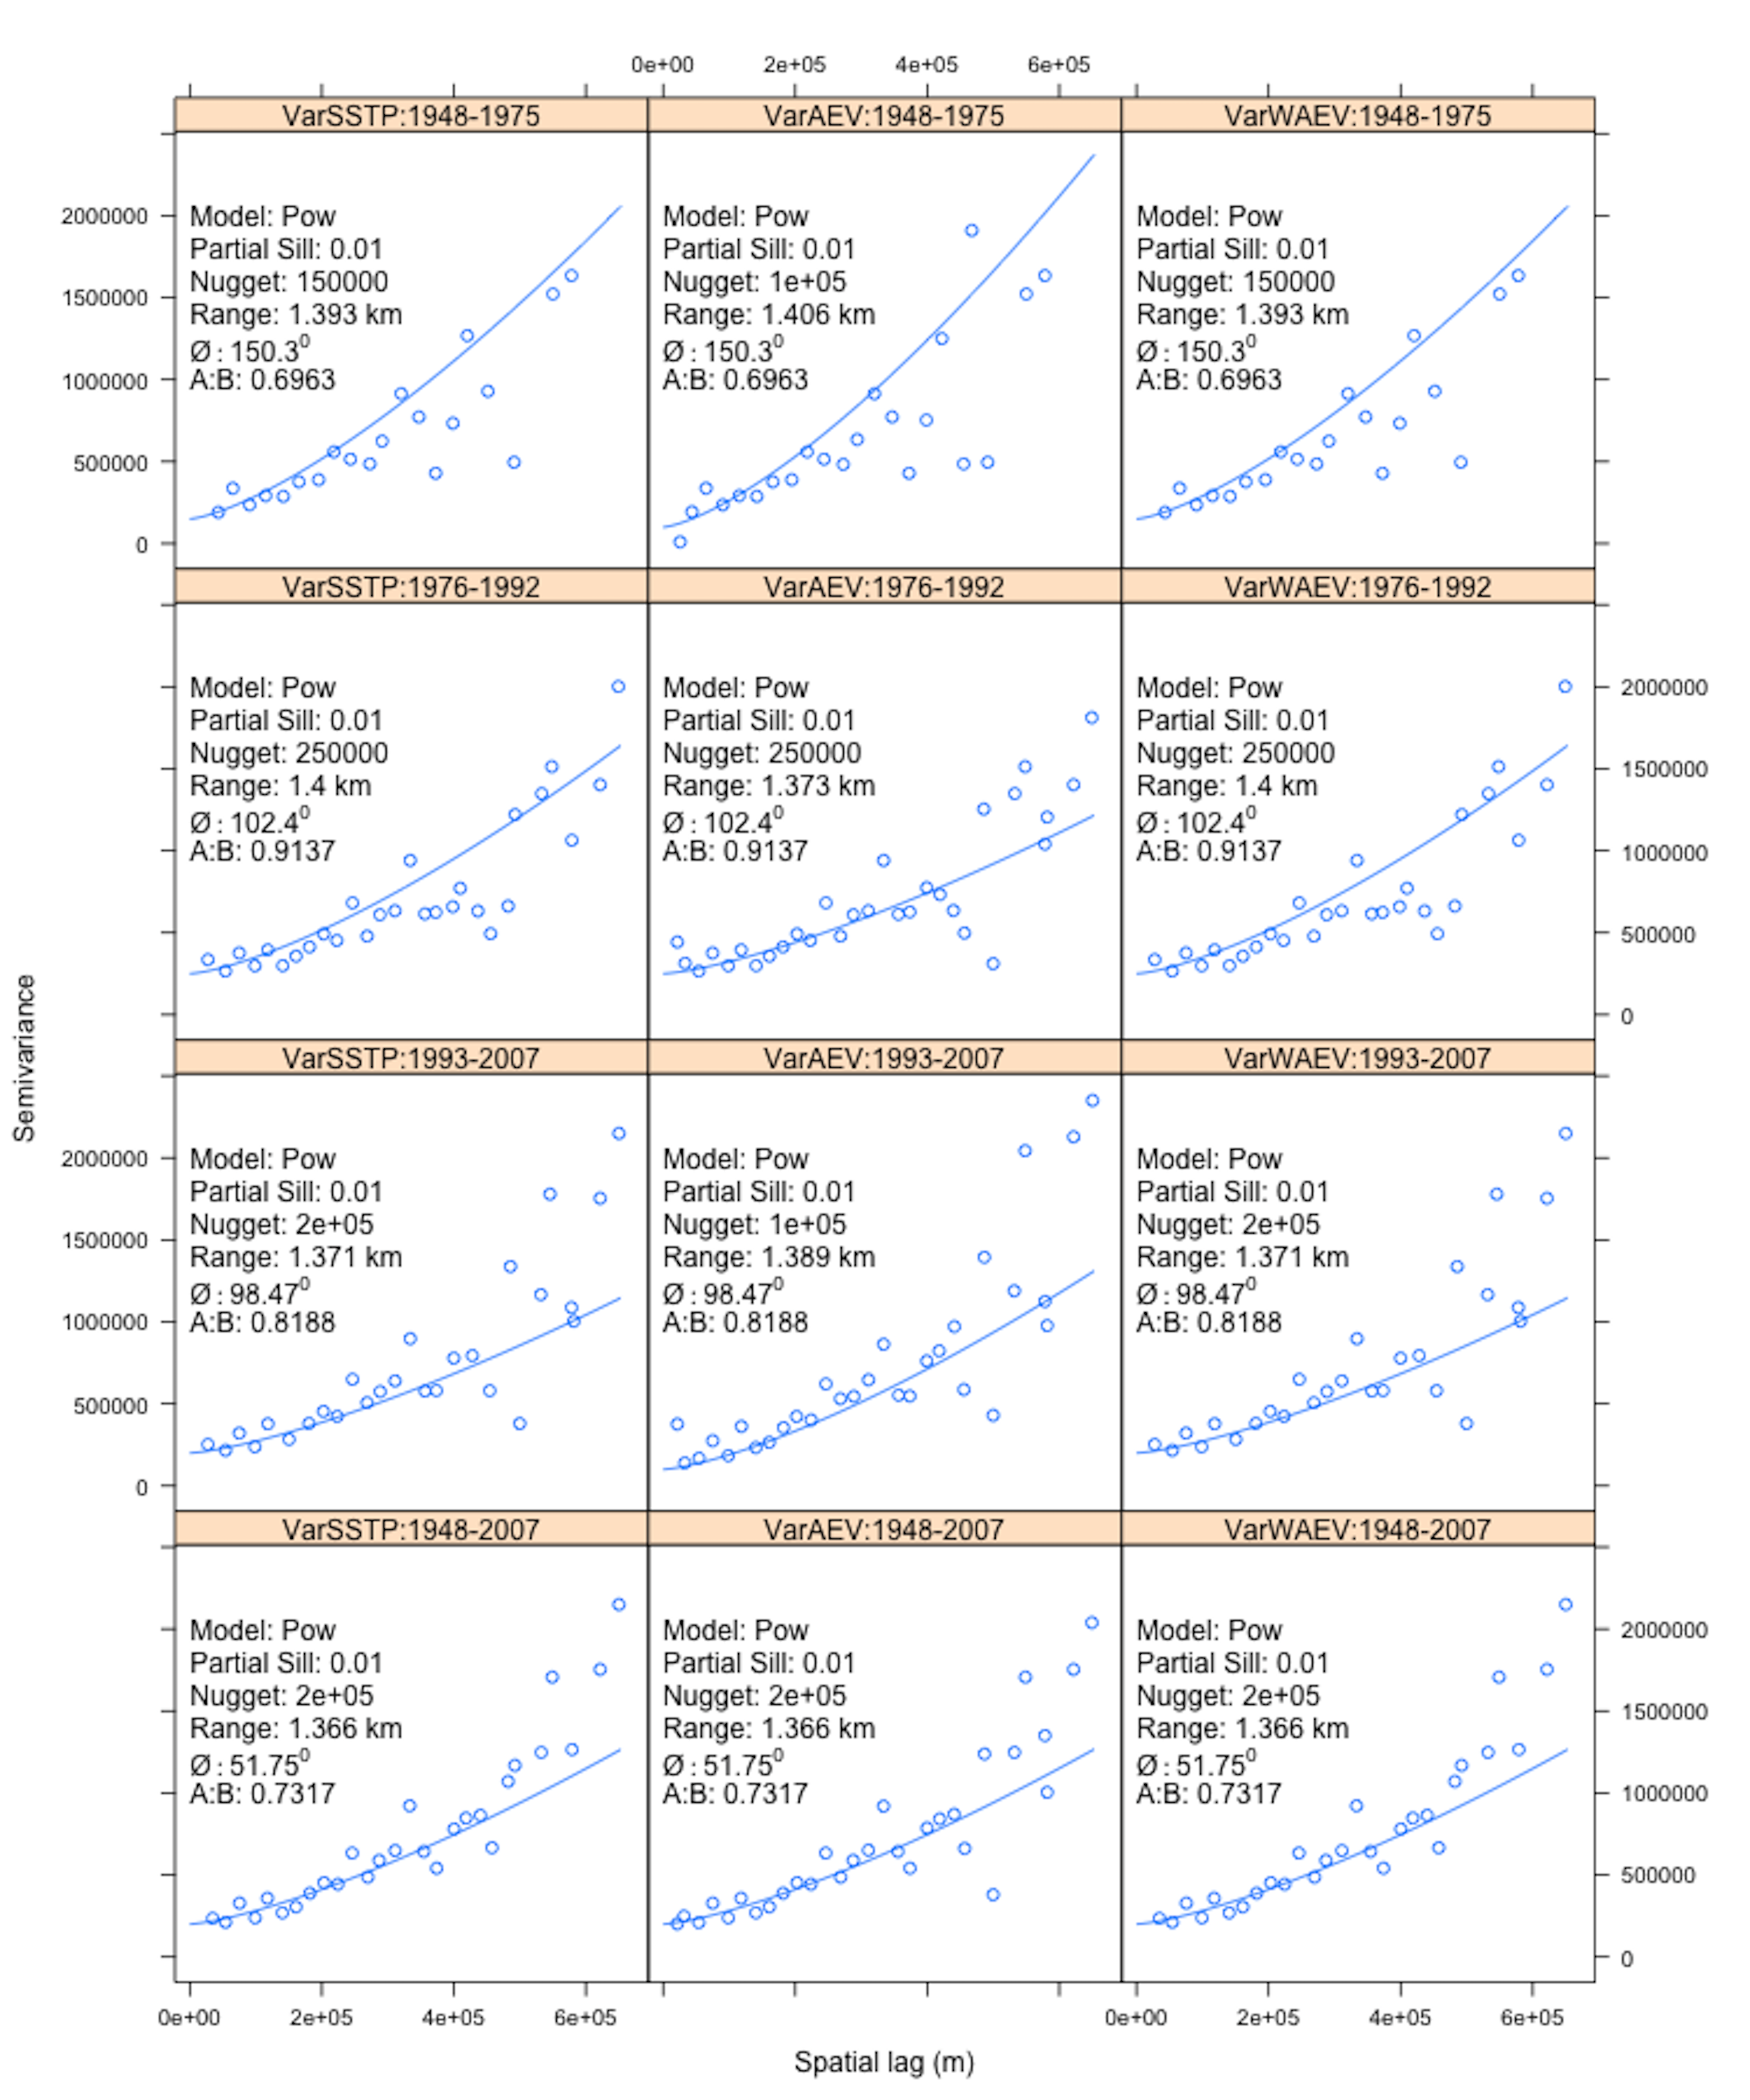
\includegraphics[width=\textwidth]{Figures/Fig_3_6.png}
  \caption{Estimated pooled within-time series (PTS) variograms (fitted best models to empirical variograms) by spatially shifting temporal points (SSTP), averaging empirical variograms (AEV) and weighted averaging empirical variograms (WAEV) methods. Figure captions depict variogram(Var) estimation method: pooled series. The “Power” (Pow) model was fitted according to $\gamma(||s_i-s_j||,\phi)=c_o+c_w||s_i-s_j||^a$, respectively, where $||s_i-s_j||$ represents the spatial lag between point pair $s_i$ and $s_j$, $\phi$ is anisotropy angle, $c_0$, $c_w$ and $a$ are nugget, partial sill variances, and range, respectively. Further details on the variogram models and their formularization and fitting in the gstat package of R are available in Cressie (1983) and Pebesma (2001). In case that anisotropy was identified, anisotropy angle ($\phi$) and the ratio between major and minor axes of the anisotropy ellipse ($A:B$) are presented.}
  \label{Fig_3_6}
\end{figure}

\clearpage

\noindent can comply with the threshold for precise isotropic (100) and anisotropic (250) variogram estimation (Webster and Oliver, 1992, 2007). For example, Laaha et al. (2013) achieved satisfactorilly precise variograms for river temperatures in Austria using 214 stations. Nevertheless, isotropic variograms were estimated with less than 100 data points in some regions for geostatistical interpolation of flood (Archfield et al., 2013), low-flow indices (Castiglioni et al., 2011) and precipitation (Todini et al., 2001). These variograms should be further validated and can be imporved by estimating PTS variograms by including comparisons from multiple time steps. However, variograms should not be estimated with fewer than 50 data points as they are imprecise and are of little value for geostatistical interpolation (Webster and Oliver, 1992; 2007). Hence, variograms estimated with less than 50 data points in previous studies (Bhowmik and Cabral, 2011; Bhowmik and Costa, 2012; Castellarin, 2014; Goovaerts, 2000; Pugliese et al. 2014) should be treated with caution in further analyses and geostatistical interpolation of corresponding hydrological variables. Note that, if all data points separable by a spatial-lag exhibit identical temporal patterns for a hydrological variable in a region, pooling derived increasing number of comparisons will provide only minor improvements on the individual variograms.

The PTS variograms also allowed for increasing data density in variogram estimation and thus increasing the smallest-spatial-lags (Table 3.1). This enabled modeling spatial variability at $\leq$ 29 km distance for all time steps (constant) within the pooled series although the smallest spatial-lags available for many years, e.g. 1948-1950, were three-fold higher ($>$ 95 km) (Figure 3.3). Thus, the PTS variograms reduce uncertainties for short distant spatial variability modeling for the time steps with large spatial lags. This was done by including point pairs separable by smaller spatial-lags available in any time step with higher data density in empirical variogram computation. However, the smallest spatial-lag for which spatial variability can be modeled for a pooled series is inherently dependent on the available data density and thus availability of spatial-lags in individual time steps, i.e. at least one point pair should be separated by a small spatial-lag in a time step. For example, if the smallest spatial-lags between point pairs with available data density in all years within the 1948-1975 series were $\geq$ 100 km, spatial variability could not be modeled at $\leq$ 29 km and could only be modeled at $\geq$ 100 km. Moreover, although SSTP generally reduces uncertainties for short distant spatial variability modeling, the reduction of uncertainties for spatial prediction of hydrological variables at short distances is higher for time steps with high data density, i.e. when the variable is gauged at short distances, than the time steps with low data density, i.e. the variable is only gauged at large distances. Thus, modeling short distant spatial variability by PTS variograms can be further improved if smaller spatial-lags are available or more point pairs are available for comparison with higher data density, i.e. more point pairs in individual time steps are separable by the smallest spatial-lags (Rogelis and Werner, 2012; Schuurmans et al., 2007).

A weaker anisotropy, i.e. directional variability, was detected in the northwest-southeast direction for the 1948-1975 series than for 1976-1992 and 1993-2007 series (Figure 3.6). This is presumably because of the lower number of spatial points per year in the 1948-1975 series than in 1976-1992 and 1993-2007 series, and thus a loss of anisotropy information (Table B.1). However, higher PRCPTOT values were observed in the southeast than the northeast of Bangladesh and a high spatial variation (average CV = 42 \%) was observed for 1948-1975 series (Figure 3.3; Table B.1). Hence, it can be claimed that the anisotropy, i.e. directional variability, of PRCPTOT was equally strong for 1948-1975 series although not captured due to lower number of spatial points per year.

Modeling spatial variability across time should consider temporal dependence or autocorrelation (Christakos, 2001; Said and Dickey, 1984). PTS variograms estimated by AEV and WAEV do not account for temporal autocorrelation as the spatial variability from time steps are averaged. Although SSTP preserves temporal autocorrelation by spatialization, i.e. spatial clusters from neighboring years are closer on space than the clusters from distant years, it also excludes temporal autocorrelation for PTS variogram estimation (spatial variability is assumed to be temporally constant). Hence, future studies should include temporal autocorrelation in PTS variogram estimation by SSTP as performed by spatiotemporal variograms (Gräler et al., 2011). Inclusion of temporal autocorrelation can be achieved by weighting spatial distances using rescaled temporal distances. This will allow for using PTS variograms in modeling time series across space, e.g. estimating time series structure for an ungauged location.

Spatiotemporal variogram estimation techniques by modeling time as a separate dimension (Gräler et al., 2011) were criticized for time series with variable spatial locations and numbers of data points (Christakos, 2001; Kerry and Oliver, 2004). However, this can be empirically examined if future studies compare the precision of the spatiotemporal variograms with the SSTP variograms for time series with variable lengths.


\subsection{Conclusions}
\label{Conclusions}

We outlined spatially shifting temporal points (SSTP) that increases precision for spatial variability modeling at both short and long distances by including variability of the smallest spatial-lag within a time series and simulaneously comparing many point pairs for large distances. SSTP was developed in the freely available and open source R software environment (R Core Team, 2015), and thus ensures reproducibility and wide spread application to geostatistical interpolation for resource constraint regions, particularly developing countries (Pebesma et al., 2012). The method is also applicable to PTS variograms estimation for geostatistical interpolation of non-hydrological spatially continuous variables in data-scarce regions. Inclusion of external variables that correlate with the variable for interpolation, e.g. elevation with precipitation (although did not correlate in our case), will increase the precision of PTS variogram estimation by SSTP (Diodato, 2005; Pebesma, 2006). To conclude, SSTP method can be further improved by integrating with the expert elicitation technique (Truong et al., 2013). 

\begingroup
\renewcommand{\addcontentsline}[3]{}% Remove functionality of \addcontentsline

\begin{thebibliography}

\bibitem{} \hangindent=1cm Archfield, S. A., Pugliese, A., Castellarin, A., Skøien, J. O., Kiang, J. E.: Topological and Canonical Kriging for Design Flood Prediction in Ungauged Catchments: An Improvement over a Traditional Regional Regression Approach?, Hydrol. Earth Syst. Sci., 17, 1575–88, doi:10.5194/hess-17-1575-2013, 2013.

\bibitem{} \hangindent=1cm Bhowmik, A.: A Comparison of Bangladesh Climate Surfaces from the Geostatistical Point of View, ISRN Met., 2012, 353408, doi:10.5402/2012/353408, 2012.

\bibitem{} \hangindent=1cm Bhowmik, A., Cabral, P.: Statistical Evaluation of Spatial Interpolation Methods for Small-Sampled Region: A Case Study of Temperature Change Phenomenon in Bangladesh, in: Computational Science and its Applications - ICCSA 2011: Lecture Notes in Computer Science, Springer, Heidelberg, Dordrecht, London, New York, 44-59, doi:10.1007/978-3-642-21928-3_4, 2011.

\bibitem{} \hangindent=1cm Bhowmik, A., Costa, A.: A Geostatistical Approach to the Seasonal Precipitation Effect on Boro Rice Production in Bangladesh, Int. J. Geosci. 3, 443-462, doi:10.4236/ijg.2012.33048, 2012.

\bibitem{} \hangindent=1cm Bhowmik, A., Costa, A.: Representativeness impacts on accuracy and precision of climate spatial interpolation in data-scarce regions. Met. Apps., doi:10.1002/met.1463, 2014.

\bibitem{} \hangindent=1cm Carrera-Hernández, J., Gaskin, S.: Spatio temporal analysis of daily precipitation and temperature in the Basin of Mexico, J. Hydro. 336, 231-249, doi:10.1016/j.jhydrol.2006.12.021, 2007.

\bibitem{} \hangindent=1cm Castellarin, A.: Regional Prediction of Flow-Duration Curves Using a Three- Dimensional Kriging, J Hydrol, 513, 179–91, doi:10.1016/j.jhydrol.2014.03.050, (2014).

\bibitem{} \hangindent=1cm Castiglioni, S., Castellarin, A., Montanari, A., Skøien, J. O., Laaha, G., Blöschl, G.: Smooth Regional Estimation of Low-Flow Indices: Physiographical Space Based Interpolation and Top-Kriging, Hydrol. Earth Syst. Sc., 15, 715–27, doi:10.5194/hess-15-715- 2011, 2011.

\bibitem{} \hangindent=1cm Christakos, G.: Modern Spatiotemporal Geostatistics, Oxford University Press, New York, 2001.

\bibitem{} \hangindent=1cm Cressie, N.: Statistics for spatial data, Revised edition, John Wiley & Sons, New York, Chichester, Toronto, Brisbane, Singapore, 1993.

\bibitem{} \hangindent=1cm Diodato, N.: The influence of topographic co-variables on the spatial variability of precipitation over small regions of complex terrain, Int. J. Clim. 25, 351-363, doi:10.1002/joc.1131, 2005.

\bibitem{} \hangindent=1cm DMICCDMP. Disaster Management Information Center of Comprehensive Disaster Management Program: Bangladesh Meteorological Department, http://www.bmd.gov.bd/index.php, last access: 25 July 2014.

\bibitem{} \hangindent=1cm Durão, R., Pereira, M., Costa, A., Côrte-Real, J., Soares, A.: Indices of precipitation extremes in southern Portugal – a geostatistical approach. Nat. Haz. E. Sys. Sci., 9, 241-250, doi:10.5194/nhess-9-241-2009, 2009.

\bibitem{} \hangindent=1cm Goovaerts, P.: Geostatistical approaches for incorporating elevation into the spatial interpolation of rainfall, J. Hydro., 228, 113-129, doi:10.1016/S0022-1694(00)00144-X, 2000.

\bibitem{} \hangindent=1cm Gräler, B., Gerharz, L., Pebesma, E.: Spatio-temporal analysis and interpolation of PM10 measurements in Europe. European Topic Center on Air Pollution and Climate Change Mitigation, Technical paper 2011/10, 2011.

\bibitem{} \hangindent=1cm Haberlandt, U.: Geostatistical interpolation of hourly precipitation from rain gauges and radar for a large-scale extreme rainfall event, J. Hydro. 332, 144-157, doi:10.1016/j.jhydrol.2006.06.028, 2007.

\bibitem{} \hangindent=1cm Kerry, R., Oliver, M.: Average variograms to guide soil sampling. Int. J. App. E. Ob. Geoinf., 5, 307–325, doi:10.1016/j.jag.2004.07.005, 2004.

\bibitem{} \hangindent=1cm Kiely, G., Albertson, J., Parlange, M.: Recent trends in diurnal variation of precipitation at valentina on the West Coast of Ireland, J. Hydro., 207, 270–279, 1998.

\bibitem{} \hangindent=1cm Kravchenko, A.: Influence of spatial structure on accuracy of interpolation methods, Soil. Sci. Soc. Am. J., 67, 1564-1571, doi:10.2136/sssaj2003.1564, 2003.

\bibitem{} \hangindent=1cm Laaha, G., Skøien, J. O. Nobilis, F., Blöschl, G.: Spatial Prediction of Stream Temperatures Using Top-Kriging with an External Drift, Env. Mod. Assess., 18, 671–83, doi:10.1007/s10666-013-9373-3, 2013.

\bibitem{} \hangindent=1cm Marchant, B., Lark, R.: Robust estimation of the variogram by residual maximum likelihood. Geoderma, 140, 62–72, doi: 10.1016/j.geoderma.2007.03.005, 2007.

\bibitem{} \hangindent=1cm Oliver, M.: The Variogram and Kriging, in: Handbook of Applied Spatial Analysis, Springer-Verlag, Berlin, Heidelberg, doi: 10.1007/978-3-642-03647-7_17, 2010.

\bibitem{} \hangindent=1cm Parajka, J., Merz, R., Skøien, J.O., Viglione, A.: The role of station density for predicting daily runoff by top-kriging interpolation in Austria, J. Hydrol. Hydromech., 63, doi: 10.1515/johh-2015-0024, 2015.

\bibitem{} \hangindent=1cm Pebesma, E. J.: Gstat user’s manual, Department of Physical Geography, Utrecht University, Utrecht, The Netherlands, Available from: http://www.gstat.org/gstat.pdf, 2001.

\bibitem{} \hangindent=1cm Pebesma, E.: Multivariable geostatistics in S: the gstat package, Comp. Geosci., 30, 683-691, doi: 10.1016/j.cageo.2004.03.012, 2004.

\bibitem{} \hangindent=1cm Pebesma, E.: The role of external variables and GIS databases in geostatistical analysis. Trans. GIS, 10, 615–632, doi: 10.1111/j.1467-9671.2006.01015.x, 2006.

\bibitem{} \hangindent=1cm Pebesma, E.: spacetime: Spatio-Temporal Data in R, J. Stat. Soft. 51, 1-30, 2012.

\bibitem{} \hangindent=1cm Pebesma, E., Cornford, D., Dubois, G., Heuvelink, G., Hristopulos, D., Pilz, J., Stöhlkerg, U., Morin, G., Skøien, J.: INTAMAP: The design and implementation of an interoperable automated interpolation web service, Comp. Geosci., 37, 343–352, doi:10.1016/j.cageo.2010.03.019, 2011.

\bibitem{} \hangindent=1cm Pebesma, E., Gräler, B.: Spatio-temporal geostatistics using gstat, available at: http://cran.r-project.org/web/packages/gstat/index.html, 2014.

\bibitem{} \hangindent=1cm Pebesma, E., Nüst, D., Bivand, R.: The R software environment in reproducible geoscientific research, Eos, Trans. A.G.U., 93, 163–163, doi: 10.1029/2012EO160003, 2012.

\bibitem{} \hangindent=1cm Peterson, T., Folland, C., Gruza, G., Hogg, W., Mokssit, A., Plummer, N.: Report on the activities of the Working Group on Climate Change Detection and Related Rapporteurs 1998–2001, Report WCDMP-47, WMO-TD 1071, World Meteorological Organization, Geneva, 2001.

\bibitem{} \hangindent=1cm Pugliese, A., Castellarin, A., Brath, A.: Geostatistical Prediction of Flow–duration Curves in an Index-Flow Framework, Hydrol. Earth Syst. Sci., 18, 3801–16, doi:10.5194/hess-18-3801-2014, 2014.

\bibitem{} \hangindent=1cm R Core Team, R: A language and environment for statistical computing, R Foundation for Statistical Computing, Vienna, available at: http://www.R-project.org, 2015.

\bibitem{} \hangindent=1cm Rogelis, M., Werner, M.: Spatial Interpolation for Real-Time Rainfall Field Estimation in Areas with Complex Topography. J. Hydromet. 14, 85-104, doi:10.1175/JHM-D-11-0150.1, 2012.

\bibitem{} \hangindent=1cm Ross, G.: Parametric and Nonparametric Sequential Change Detection in R: The cpm package, J. Stat. Soft., in press, 2014.

\bibitem{} \hangindent=1cm Said, S., Dickey, D.: Testing for Unit Roots in Autoregressive-Moving Average Models of Unknown Order, Biometrika, 71, 599–607, doi:10.1093/biomet/71.3.599, 1984.

\bibitem{} \hangindent=1cm Schuurmans, J., Bierkens, M., Pebesma, E.: Automatic Prediction of High-Resolution Daily Rainfall Fields for Multiple Extents: The Potential of Operational Radar, J. Hydromet. 8, 1204-1224, doi:10.1175/2007JHM792.1, 2007.

\bibitem{} \hangindent=1cm Skøien, J. O., Merz, R., Blöschl, G.: Top-kriging-geostatistics on stream networks, Hydrol. Earth Syst. Sci., 10, 277–287, doi:10.5194/hess-10-277-2006, 2006.

\bibitem{} \hangindent=1cm Skøien, J. O., Blöschl, G., Laaha, G., Pebesma, E., Parajka, J., Viglione, A.: rtop: an R package for interpolation of data with a variable spatial support, with an example from river networks, Comp. Geosci., doi:10.1016/j.cageo.2014.02.009, 2014.

\bibitem{} \hangindent=1cm Skøien, J. O., Pebesma, E. J., Blöschl, G.: Geostatistics for automatic estimation of environmental variables—some simple solutions, Georisk, 2, 259–272, doi:10.1080/17499510802086769, 2008.

\bibitem{} \hangindent=1cm Stocker, T., Dahe, Q., Plattner, G.: Climate Change 2013: The Physical Science Basis, Working Group I Contribution to the Fifth Assessment Report of the Intergovernmental Panel on Climate Change, Summary for Policymakers, Intergovernmental Panel on Climate Change (IPCC), 2013.

\bibitem{} \hangindent=1cm Todini, E., Pellegrini, F., Mazzetti, C.: Influence of Parameter Estimation Uncertainty in Kriging: Part 2 - Test and Case Study Applications, Hydrol. Earth Syst. Sci., 5, 225–32, doi:10.5194/hess-5-225-2001, 2001.

\bibitem{} \hangindent=1cm Truong, P., Heuvelink, G., Gosling, J.: Web-based tool for expert elicitation of the variogram. Comp. Geosci., 51, 390–399, doi:10.1016/j.cageo.2012.08.010, 2013.

\bibitem{} \hangindent=1cm Wagner, P., Fiener, P., Wilken, F., Kumar, S., Schneider, K.: Comparison and evaluation of spatial interpolation schemes for daily rainfall in data scarce regions, J. Hydro., 464-465, 388-400, doi:10.1016/j.jhydrol.2012.07.026, 2012.

\bibitem{} \hangindent=1cm Webster, R., Oliver, M.: Sample adequately to estimate variograms of soil properties, J. Soil. Sci., 43, 177-192, doi:10.1111/j.1365-2389.1992.tb00128.x, 1992.

\bibitem{} \hangindent=1cm Webster, R., Oliver, M.: Geostatistics for Environmental Scientists, John Wiley and Sons Ltd., Chichester, 2007.

\end{thebibliography}

\endgroup